\documentclass[a4paper]{scrbook}

\usepackage[utf8]{inputenc}
\usepackage{graphicx}
\usepackage{booktabs}
\usepackage{url}
\usepackage{relsize}
\usepackage{hyperref}
\usepackage{libertine}
\usepackage{ifthen}
\usepackage{float}
\usepackage{enumerate}
\usepackage{enumitem}
\usepackage{tabularx}
\usepackage{adjustbox}
\usepackage{amsmath,amssymb,amsfonts}
\usepackage{setspace}
\usepackage{caption}
\usepackage{subcaption}
\usepackage{xcolor}
\usepackage{cite} 
\usepackage{algorithm}
\usepackage{algpseudocode}
\usepackage{array}
\usepackage{textcomp}
\usepackage{anyfontsize}
\usepackage{pifont}
\usepackage{amssymb} 
\usepackage{pgfplots}
\usepackage{listings}
\usepackage{colortbl}
\usepackage{rotating}   % for \rotatebox
\usepackage{pdflscape}
\usepackage{placeins}   % for \FloatBarrier
\usepackage{multirow}
\usepackage{svg}

\usepackage{ragged2e}
\newcolumntype{Y}{>{\RaggedRight\arraybackslash}X}


\pgfplotsset{compat=1.18}


\lstset{
    language=Python,
    basicstyle=\ttfamily\small,
    keywordstyle=\color{blue},
    stringstyle=\color{orange},
    commentstyle=\color{gray},
    frame=single,
    breaklines=true,
    columns=flexible,
    backgroundcolor=\color{gray!5},
    captionpos=b
}



\onehalfspacing  
\KOMAoptions{open=any}


% \usepackage{cite} 

\raggedbottom
% \usepackage{fancyhdr}
% \KOMAoptions{open=any}


%%%%%%%%%%%%%%%%%%%%%%%%%%%%%%%%%%%%%%%%%%%%%%%%%%%%%%%%%%%%%%%%%%%%%%%%%%%%%%%%
% Replace these values
%%%%%%%%%%%%%%%%%%%%%%%%%%%%%%%%%%%%%%%%%%%%%%%%%%%%%%%%%%%%%%%%%%%%%%%%%%%%%%%%
\newcommand{\thesistitleEN}{Development and Evaluation of an AI-Based Real-Time Interpretation System with a Feasibility Study on Hardware Integration}
\newcommand{\thesistitleDE}{Entwicklung und Evaluation eines KI-basierten Echtzeit-Dolmetschsystems mit einer Machbarkeitsstudie zur Hardware-Integration}

\newcommand{\student}{Abdelrahman Mohamed}
\newcommand{\matrnr}{22201965}
\newcommand{\stammnr}{} % Unset this variable if you only have a (single) matriculation number
% \newcommand{\stammnr}{234567} % Unset this variable if you only have a (single) matriculation number
\newcommand{\submissiondate}{15.\ January 2025}
\newcommand{\supervisor}{Prof. Dr. Patrick Glauner}
\newcommand{\secsupervisor}{} % Unset this variable if no second supervisor is required
% \newcommand{\secsupervisor}{Prof.~Dr.~Zweitprüfer} % Unset this variable if no second supervisor is required
\newcommand{\faculty}{Faculty of Computer Science}

% Select your course of studies here
\newcommand{\studies}{Bachelor Artificial Intelligence}
\newcommand{\degree}{Bachelor of Science (B.Sc.)}
%%%%%%%%%%%%%%%%%%%%%%%%%%%%%%%%%%%%%%%%%%%%%%%%%%%%%%%%%%%%%%%%%%%%%%%%%%%%%%%%

\renewcommand*{\UrlFont}{\ttfamily\smaller\relax}

\begin{document}
\pagestyle{headings}
\pagenumbering{roman}


% \input{declaration}
\setkomafont{title}{\Large \scshape}
\begin{titlepage}
\begin{center}
	{\usekomafont{subject}
	Deggendorf Institute of Technology\\
	  \faculty\par}
	\vspace{.2cm}
{\Large \studies\\}
% {\Large Studiengang \studies\\}
\vspace{5.5\baselineskip}
{\usekomafont{title}\thesistitleEN\par}
\vspace{1cm}
{\usekomafont{title}\thesistitleDE\par}
\vspace{5.5\baselineskip}

\usekomafont{publishers}
Bachelor thesis  in fulfillment of the requirements for the degree of:
: % Bachelorarbeit zur Erlangung des akademischen Grades:

	\vspace{.2cm}
	\emph{\degree}
	\vspace{.2cm}

at the Deggendorf Institute of Technology\\
\end{center}
\vfill
\parbox[t]{.47\textwidth}{\usekomafont{author}
	Submitted by:\\
	\student\\
	Matriculation Number: \matrnr\par
	\ifthenelse{\equal{\stammnr}{}}{}{
	Stammnummer: \stammnr\par
	}
    \vspace{.5cm}
	On: \submissiondate\par
}
\hfill
\parbox[t]{.35\textwidth}{\usekomafont{author}
Supervisor:\\
\supervisor%

\ifthenelse{\equal{\secsupervisor}{}}{}
{%
\vspace{\baselineskip}
Ergänzende Prüfende:\\
\secsupervisor%
}}
\end{titlepage}
\cleardoublepage\par
% \clearpage\par
\begingroup
\setstretch{1.0}
%\input{declaration}
\endgroup


\tableofcontents
\chapter*{List of Abbreviations}
% \addcontentsline{toc}{chapter}{List of Abbreviations}

\begin{table}[h!]
\centering
\begin{tabular}{ll}
\textbf{Abbreviation} & \textbf{Full Form} \\
\midrule
ASR      & Automatic Speech Recognition \\
NMT      & Neural Machine Translation \\
MT       & Machine Translation \\
TTS      & Text-to-Speech \\
PCM      & Pulse-code modulation \\
HTTP     & Hypertext Transfer Protocol \\
kHz      & Kilohertz \\
CCU      & Central Control Unit \\
WPM      & Words Per Minute \\
WER      & Word Error Rate   \\
CER      & Character Error Rate \\
BLEU     & BiLingual Evaluation Understudy \\
METEOR   & Metric for Evaluation of Translation with Explicit Ordering \\
BERT     & Bidirectional Encoder Representations from Transformers \\
MOS      & Mean Opinion Score \\
PESQ     & Perceptual Evaluation of Speech Quality \\
AL       & Average Lagging \\
EVS      & Ear–Voice Span \\
LAAL     & Length-Adaptive Average Lagging \\
RTF      & Real-Time Factor \\
FTL      & First-Token Latency \\
TTFA     & Time to First Audio \\
NE       & Normalized Erasure \\
CW       & Consecutive Wait \\
MU       & Meaning Unit \\
\end{tabular}
\end{table}
\listoftables
\listoffigures

% \chapter*{Abstract}
\chapter*{Abstract}

Simultaneous interpretation is a cornerstone of multilingual communication in international conferences and institutional settings, yet it traditionally relies on highly skilled human interpreters and specialized hardware infrastructures that are costly, resource-intensive, and difficult to scale. Recent advances in automatic speech recognition (ASR), neural machine translation (NMT), and text-to-speech (TTS) synthesis have made AI-based interpretation technically feasible; however, achieving reliable real-time performance remains a challenging engineering problem due to strict latency, stability, and integration constraints. This thesis investigates the design, implementation, and evaluation of a real-time AI-based simultaneous interpretation system from a system-engineering perspective. The proposed solution adopts a modular, provider-agnostic architecture that integrates streaming ASR, NMT, and TTS synthesis within a unified pipeline, with particular emphasis on incremental processing, stability-aware segmentation, asynchronous execution, and multi-language output support. The objectives are threefold: (i) to design and validate a real-time interpretation pipeline capable of processing continuous speech input with bounded end-to-end latency, (ii) to develop a system-level evaluation framework that quantifies latency and stability trade-offs, (iii) and to assess the feasibility of integrating AI-generated interpretation output into professional interpretation hardware environments. Experimental results obtained under standardized real-time conditions demonstrate that the proposed system maintains latency within acceptable bounds for simultaneous interpretation across multiple configurations, while component-level analysis highlights recognition and segmentation as the dominant contributors to delay. Ablation studies reveal non-trivial trade-offs between responsiveness and output stability, underscoring the importance of system-level orchestration. Finally, a hardware integration feasibility study shows that AI-based interpretation output can be aligned with professional channel-based audio infrastructures using standardized digital audio formats, supporting practical deployment beyond software-only demonstrations.
\addcontentsline{toc}{chapter}{Abstract}
% \cleardoublepage

\setcounter{page}{1}
\pagenumbering{arabic}


\chapter{Introduction}
\label{chapter:introduction}

Multilingual communication is a fundamental requirement in many modern contexts, including international conferences, governmental institutions, and global online events. Simultaneous interpretation plays a critical role in enabling such communication by allowing spoken content in a source language to be rendered into one or more target languages with minimal delay. Traditionally, this task has been performed by highly trained human interpreters supported by specialized audio infrastructure \cite{Seeber2015CognitiveLoad}. While this approach delivers high-quality results, it is costly, difficult to scale, and constrained by logistical and availability limitations \cite{dhawan2022speech2speechchallenges, gencheva2023features}.

Recent advances in artificial intelligence have opened new opportunities for automating parts of the interpretation process. Progress in automatic speech recognition, neural machine translation, and text-to-speech synthesis has made it technically feasible to construct end-to-end systems capable of transforming spoken language into translated speech in near real time \cite{popescu-belis2025s2streview}. These developments have sparked growing interest in AI-based simultaneous interpretation systems that aim to reduce operational costs, improve accessibility, and support multilingual communication at scale \cite{ozkaya2023transformative}.

Despite this progress, real-time AI-based interpretation remains a challenging engineering problem. Unlike offline translation or post-event transcription, simultaneous interpretation imposes strict latency requirements that directly affect usability \cite{zheng-etal-2020-fluent}. Spoken input arrives continuously, intermediate representations are inherently unstable, and delays introduced at each processing stage can accumulate rapidly. Furthermore, interpretation systems must operate reliably over extended sessions, support multiple target languages, and integrate seamlessly with audio input and output mechanisms.

Most existing AI-based interpretation approaches can be broadly categorized into either end-to-end speech-to-speech models \cite{jia2022translatotron2} or cascaded pipelines composed of separate speech recognition, translation, and synthesis components \cite{popescu-belis2025s2streview}. While end-to-end models offer conceptual simplicity, they often lack the flexibility and controllability required for real-time deployment. Cascaded architectures, on the other hand, enable modularity and practical integration but introduce challenges related to segmentation, synchronization, and stability across components. As a result, many current systems struggle to balance low latency with coherent and reliable output in live settings \cite{sperber2020endtoendpromise, Sethiya2023EndtoEndSurvey, Etchegoyhen2022CascadeDirectCase}.

In addition to algorithmic challenges, practical deployment considerations further complicate the design of real-time interpretation systems. Professional interpretation environments rely on standardized audio formats, routing mechanisms, and dedicated hardware infrastructure \cite{conference_interpreting_new_tech}. However, many AI-based solutions are developed primarily for software-only or consumer-oriented use cases \cite{dhawan2022speech2speechchallenges} , limiting their applicability in professional contexts \cite{ozkaya2023transformative}. Moreover, existing platforms are often provider-locked, restricting flexibility and hindering systematic evaluation across alternative AI services \cite{sperber2020endtoendpromise}.

Motivated by these challenges, this thesis investigates the design and implementation of a real-time AI-based simultaneous interpretation system with a strong emphasis on system architecture, latency control, and practical integration. Rather than focusing on training new models, the work adopts a system-engineering perspective that leverages state-of-the-art AI services within a unified, modular pipeline.  The work is guided by three main objectives:
\begin{enumerate}
  \item To design a real-time AI-based simultaneous interpretation pipeline that processes continuous speech input using streaming ASR, NMT, and TTS synthesis, while ensuring low end-to-end latency, stable incremental output, and support for modular, provider-agnostic, and multi-language operation.
  
  \item To develop and apply a system-level evaluation framework that quantifies the performance of the proposed pipeline, with particular emphasis on end-to-end latency, component-level delays, and the impact of segmentation parameters on translation behavior.
  
  \item To investigate the feasibility of integrating AI-based interpretation pipelines with professional interpretation hardware and audio systems, considering standardized audio formats, real-time routing requirements, and practical deployment constraints.
\end{enumerate}

The remainder of this thesis is structured as follows: 
Chapter~\ref{chapter:background} provides background information and reviews related work in traditional interpretation systems, core speech and language technologies, and existing AI-based interpretation approaches, culminating in the identification of key limitations and research gaps. 
Chapter~\ref{chapter:methodology} presents the methodology and system design, detailing the architecture of the proposed real-time interpretation pipeline, its individual components, and the evaluation framework used to assess system performance. 
Chapter~\ref{chapter:results} presents the experimental results, focusing on end-to-end latency behavior, component-level delays, and system performance under real-time conditions, while Chapter~\ref{chapter:discussion} provides a detailed discussion and interpretation of these findings.
Chapter~\ref{chapter:hardware} examines the feasibility of integrating AI-based interpretation pipelines with professional interpretation hardware and audio systems, addressing practical deployment considerations and interface requirements. 
Finally, Chapter~\ref{chapter:conclusion} concludes the thesis by summarizing the main findings and outlining directions for future work.

\chapter{Background \& Related Work}
\label{chapter:background}


\section{Traditional Simultaneous Interpretation Systems}

Simultaneous interpretation has long been a cornerstone of multilingual communication in international conferences, governmental institutions, and large-scale events. In traditional settings, interpretation is performed by highly trained human interpreters who listen to a speaker in a source language and deliver a near-synchronous spoken translation in a target language. This process requires a high level of linguistic expertise, cognitive load management, and sustained concentration, making professional interpreters a scarce and costly resource \cite{gencheva2023features}.

In addition to human expertise, traditional simultaneous interpretation relies on a specialized physical infrastructure designed to ensure low-latency audio transmission and clear separation between source and target language channels. Interpreters typically work inside sound-isolated booths, where they receive the original speech through headphones and produce the translated output via microphones. These booths are engineered to minimize external noise and prevent audio feedback, thereby maintaining translation accuracy and listener comfort.

The interpreter audio is routed through dedicated interpretation consoles that allow control over input channels, volume levels, and language selection. From there, the translated signal is transmitted using wired or wireless distribution systems to receivers used by audience members. Listeners select their preferred language channel on handheld receivers or integrated conference devices, enabling simultaneous access to multiple language streams \cite{conference_interpreting_new_tech}. The components of such a traditional interpretation setup are visualized in Figure~\ref{fig:traditional_interpretation_system}.

\begin{figure}[!htbp]
  \centering
  \includegraphics[width=\textwidth]{img/figures/traditional_interpretation_system.drawio.png}
  % \footnotemark creates the red number in the caption
  \caption[Traditional Simultaneous Interpretation System Components]{Traditional simultaneous interpretation system components. Adapted from \footnotemark}
  \label{fig:traditional_interpretation_system}
\end{figure}

% \footnotetext places the link at the bottom of the current page
\footnotetext{\url{https://media.boschsecurity.com/fs//media/pt/pb/media/products_1/conference_systems_1/integrus_brochure.pdf}}

This tightly integrated hardware ecosystem ensures reliable, low-latency delivery of interpreted speech but comes with significant logistical requirements \cite{ozkaya2023transformative}. Deploying a traditional interpretation system involves transporting and installing booths, consoles, transmitters, receivers, and cabling, often requiring specialized technicians. Furthermore, each additional target language increases system complexity, as it necessitates additional interpreters, booths, and audio channels. As a result, scalability is limited, particularly for events with many languages or dynamically changing interpretation needs.

From an economic perspective, traditional simultaneous interpretation incurs substantial recurring costs. These include interpreter fees, equipment rental, installation labor, and on-site technical support. Such costs can be prohibitive for smaller organizations or informal settings, restricting access to high-quality multilingual communication. Moreover, reliance on physical infrastructure constrains deployment flexibility, making rapid or remote interpretation scenarios difficult to support \cite{rayaa2022remoteSI}.

Despite these limitations, traditional interpretation systems remain the industry standard due to their proven reliability and high output quality. They therefore provide an important baseline against which alternative approaches must be evaluated. In particular, any AI-based interpretation system aiming for real-world applicability must account for similar requirements in terms of latency, audio routing, and hardware compatibility \cite{dhawan2022speech2speechchallenges}. The feasibility of integrating AI-driven interpretation pipelines with professional audio equipment is therefore a critical consideration and is revisited later in this thesis in Section~\ref{chapter:hardware}.


\section{Core Technologies for Real-Time Speech Interpretation}

This section provides background on the core technologies that underpin modern real-time speech interpretation systems. In particular, it reviews the roles and operational characteristics of Automatic Speech Recognition, Neural Machine Translation, and Text-to-Speech synthesis when deployed under strict real-time constraints. Rather than focusing on model architectures or training methodologies, the discussion emphasizes streaming behavior, latency considerations, and system-level challenges that arise when these components are combined into an end-to-end interpretation pipeline. This technological foundation establishes the context for the system design choices presented in Chapter~\ref{chapter:methodology}.

\subsection{Automatic Speech Recognition in Streaming Settings}

Automatic Speech Recognition (ASR) refers to the process of converting spoken language into written text using computational systems \cite{nayeem2025asr_survey}. In the context of multilingual communication, ASR serves as the primary interface between continuous audio input and downstream language processing components \cite{8252104}. For real-time speech interpretation, ASR systems must operate under strict temporal constraints, producing textual output incrementally as speech unfolds rather than after complete utterances are available. A comparison between batch-based and streaming automatic speech recognition, highlighting incremental processing and partial hypothesis generation in streaming settings is visualised in Figure~\ref{fig:streaming_vs_batch_asr}.

\begin{figure}[!htbp]
  \centering
  \includesvg[width=\textwidth]{img/figures/streaming_vs_batch_asr.drawio.svg}
  \caption[Batch-based and Streaming Automatic Speech Recognition Comparison]{Batch-based and Streaming Automatic Speech Recognition Comparison}
  \label{fig:streaming_vs_batch_asr}
\end{figure}

Traditional ASR systems have often been designed for batch or offline processing, where an entire audio recording is first captured and then transcribed in a single pass. While such approaches can leverage full acoustic context to improve transcription accuracy, they introduce delays that are incompatible with simultaneous interpretation scenarios. In contrast, streaming ASR systems process audio input continuously and emit recognition results in near real time. This distinction is fundamental for applications that require immediate downstream processing, such as live translation or captioning.

A defining characteristic of streaming ASR is the generation of partial hypotheses. As audio is processed incrementally, the recognizer produces provisional text outputs that may be revised as additional acoustic context becomes available. These partial hypotheses allow downstream components to react early to spoken content, thereby reducing overall latency. However, they also introduce instability, as previously emitted text segments may change or be retracted. Streaming ASR systems therefore balance two competing objectives: minimizing latency while maintaining sufficient stability in the generated transcripts \cite{weller2021streamingST}.

In real-time interpretation settings, this trade-off between responsiveness and stability becomes particularly critical. Partial hypotheses that are forwarded too aggressively may lead to semantic inconsistencies or repeated processing in downstream stages. Conversely, delaying output until hypotheses are fully stable increases end-to-end latency and undermines the simultaneity of interpretation \cite{grissom2014realtime}. As a result, streaming ASR is not merely a faster variant of offline recognition but a qualitatively different operating mode with distinct design considerations.

Another important distinction between streaming and batch ASR lies in how speech boundaries are handled. Offline systems can rely on explicit sentence boundaries or complete utterances, whereas streaming systems must operate without prior knowledge of sentence length or structure. Instead, they infer boundaries implicitly from acoustic cues, pauses, or internal confidence measures \cite{weller2021streamingST}. This behavior directly affects how recognized speech can be segmented and forwarded for translation in real time.

From a system perspective, streaming ASR is typically integrated as a continuous service that accepts audio chunks of fixed duration and returns updated recognition hypotheses asynchronously. This incremental interaction model enables low-latency processing but requires careful coordination with downstream components that consume ASR output. In particular, downstream stages must be designed to tolerate hypothesis revisions and to distinguish between provisional and finalized recognition results.


\subsection{Neural Machine Translation for Spoken Language}

Neural Machine Translation (NMT) refers to the use of neural network–based models to automatically translate text from a source language into a target language \cite{stahlberg2020nmt_review}. In contrast to earlier rule-based or statistical approaches, modern NMT systems model translation as a sequence-to-sequence transformation and have become the dominant paradigm in both academic research and commercial deployment. Within real-time speech interpretation systems, NMT serves as the core linguistic transformation stage that converts recognized speech content into translated text suitable for immediate delivery or speech synthesis \cite{sperber2020endtoendpromise}.

Most established NMT systems are designed for text-based translation scenarios, such as documents, subtitles, or conversational messages, where complete sentences or paragraphs are available prior to translation. In such settings, the translation model can leverage full contextual information, including sentence boundaries and long-range dependencies, to maximize output quality. However, real-time interpretation imposes fundamentally different constraints. Instead of well-formed textual input, NMT systems receive short, incrementally generated speech segments that may represent incomplete clauses or evolving utterances \cite{chen2024metamorphosisMT}.

This distinction between document-level text translation and speech segment translation has important implications. In spoken language interpretation, translation must often be performed on partial and temporally constrained input, without access to the full sentence context. As a result, translation decisions are made under uncertainty, and the system must balance early output generation against the risk of semantic incompleteness. These constraints differentiate real-time NMT from traditional text translation tasks and require system-level strategies that prioritize responsiveness alongside linguistic coherence.

A central challenge in spoken-language NMT is the trade-off between latency and translation quality. Translating shorter segments reduces delay and improves simultaneity but may degrade fluency or lead to awkward phrasing due to missing context. Conversely, aggregating longer segments can improve translation accuracy but increases end-to-end latency, which is undesirable in live interpretation scenarios. This trade-off is inherent to real-time systems and cannot be resolved solely through model improvements; instead, it must be managed through careful segmentation and pipeline design.

Segment-based translation introduces additional challenges related to consistency and continuity. Since continuous segments are translated instantly in a connected stream, maintaining coherent terminology, pronoun references, and discourse flow across segments becomes more difficult than in document-level translation \cite{dhawan2022speech2speechchallenges}. Furthermore, variations in segment length and timing can lead to uneven translation pacing, which must be handled gracefully by downstream components such as text-to-speech synthesis. These challenges highlight the importance of viewing NMT as one component within a broader real-time system rather than as an isolated module.

Despite these limitations, segment-level NMT remains the most practical approach for real-time interpretation due to its compatibility with streaming pipelines and asynchronous execution models. By translating speech incrementally, systems can deliver translated content with minimal delay while preserving acceptable semantic quality. As summarized in Table~\ref{tab:nmt_text_vs_speech}, the operational requirements of spoken-language translation differ substantially from those of traditional text translation, motivating specialized system-level adaptations for real-time use cases.


\begin{table}[!htbp]
  \centering
  \caption[Text translation and segment-based translation comparison]{Comparison between document-level text translation and segment-based translation for spoken language}
  \label{tab:nmt_text_vs_speech}
  \begin{adjustbox}{max width=\textwidth, keepaspectratio=false}
    \begin{tabular}{p{4.3cm} p{7.5cm} p{7.5cm}}
      \toprule
      \textbf{Aspect} & \textbf{Text Translation} & \textbf{Spoken-Language Translation} \\
      \midrule
      Input characteristics 
      &
      \begin{itemize}[nosep,leftmargin=*]
        \item Complete sentences or full documents
        \item Static input available before translation
        \item Explicit sentence boundaries
      \end{itemize}
      &
      \begin{itemize}[nosep,leftmargin=*]
        \item Incremental speech segments
        \item Input evolves over time
        \item Implicit and dynamically inferred boundaries
      \end{itemize} \\
      \midrule
      Context availability 
      &
      \begin{itemize}[nosep,leftmargin=*]
        \item Global context across sentences or paragraphs
        \item Long-range dependencies accessible
        \item Stable discourse structure
      \end{itemize}
      &
      \begin{itemize}[nosep,leftmargin=*]
        \item Limited local context
        \item Partial or incomplete semantic information
        \item No access to future utterances
      \end{itemize} \\
      \midrule
      Latency requirements 
      &
      \begin{itemize}[nosep,leftmargin=*]
        \item Latency typically non-critical
        \item Offline or asynchronous processing acceptable
        \item Quality prioritized over speed
      \end{itemize}
      &
      \begin{itemize}[nosep,leftmargin=*]
        \item Strict real-time constraints
        \item Low end-to-end delay required
        \item Latency directly affects usability
      \end{itemize} \\
      \midrule
      Translation granularity 
      &
      \begin{itemize}[nosep,leftmargin=*]
        \item Sentence-level or paragraph-level units
        \item Coherent, complete linguistic structures
      \end{itemize}
      &
      \begin{itemize}[nosep,leftmargin=*]
        \item Clause-level or short segment-level units
        \item Semantically incomplete fragments possible
      \end{itemize} \\
      \midrule
      Stability and revision risk 
      &
      \begin{itemize}[nosep,leftmargin=*]
        \item No revision after translation
        \item Input text remains unchanged
      \end{itemize}
      &
      \begin{itemize}[nosep,leftmargin=*]
        \item Risk of revision due to evolving speech
        \item Dependence on ASR hypothesis stability
      \end{itemize} \\
      \bottomrule
    \end{tabular}
  \end{adjustbox}
\end{table}

\vspace{3cm}
\subsection{Text-to-Speech in Live Interpretation Scenarios}

Text-to-Speech (TTS) systems are responsible for converting textual representations of language into intelligible spoken audio \cite{tan2021tts_survey}. In the context of real-time speech interpretation, TTS constitutes the final stage of the processing pipeline, directly affecting the listener’s perception of responsiveness, fluency, and overall system quality. Unlike offline speech synthesis applications, live interpretation imposes strict constraints on latency and audio delivery, requiring TTS systems to operate incrementally and with minimal delay.

In traditional applications such as audiobook narration or voice assistants, speech synthesis can be performed on complete sentences or paragraphs, allowing models to optimize for prosody, expressiveness, and naturalness. However, in simultaneous interpretation, TTS systems receive short, segment-level translation outputs that may represent incomplete clauses or evolving utterances. As a result, synthesis must begin promptly upon receiving each segment, even when full linguistic context is unavailable \cite{popescu-belis2025s2streview}. This operational mode fundamentally differentiates live interpretation TTS from conventional speech synthesis tasks.

Historically, TTS systems were based on concatenative or parametric approaches, which relied on pre-recorded speech units or handcrafted acoustic models. While these methods offered predictable latency and low computational overhead, they often produced unnatural or monotonous speech \cite{cohn2020perceptionTTS}. Recent advances in neural TTS have significantly improved naturalness and speaker expressiveness, enabling synthetic speech that closely resembles human voices. These improvements have facilitated the adoption of neural TTS in real-time applications, including interpretation systems, despite their higher computational complexity \cite{cohn2020perceptionTTS}. To highlight the differences between traditional and neural text-to-speech approaches in the context of live interpretation, Table~\ref{tab:tts_traditional_vs_neural} summarizes their key characteristics with respect to latency, naturalness, and real-time suitability.

\begin{table}[!htbp]
  \centering
  \caption[Traditional and neural TTS comparison]{Comparison between traditional and neural text-to-speech approaches in live interpretation scenarios}
  \label{tab:tts_traditional_vs_neural}
  \begin{adjustbox}{max width=\textwidth, keepaspectratio=false}
    \begin{tabular}{p{4.3cm} p{7.5cm} p{7.5cm}}
      \toprule
      \textbf{Aspect} & \textbf{Traditional TTS} & \textbf{Neural TTS} \\
      \midrule
      Synthesis approach
      &
      \begin{itemize}[nosep,leftmargin=*]
        \item Concatenative or parametric methods
        \item Predefined acoustic units
        \item Limited modeling of prosody
      \end{itemize}
      &
      \begin{itemize}[nosep,leftmargin=*]
        \item Data-driven neural models
        \item End-to-end acoustic modeling
        \item Improved prosody and expressiveness
      \end{itemize} \\
      \midrule
      Speech naturalness
      &
      \begin{itemize}[nosep,leftmargin=*]
        \item Robotic or monotonous output
        \item Limited speaker variation
      \end{itemize}
      &
      \begin{itemize}[nosep,leftmargin=*]
        \item Human-like speech quality
        \item Multiple voices and speaking styles
      \end{itemize} \\
      \midrule
      Latency characteristics
      &
      \begin{itemize}[nosep,leftmargin=*]
        \item Predictable and low synthesis delay
        \item Suitable for strict real-time constraints
      \end{itemize}
      &
      \begin{itemize}[nosep,leftmargin=*]
        \item Higher computational cost
        \item Requires latency-aware configuration
      \end{itemize} \\
      \midrule
      Suitability for live interpretation
      &
      \begin{itemize}[nosep,leftmargin=*]
        \item High responsiveness
        \item Limited listener comfort
      \end{itemize}
      &
      \begin{itemize}[nosep,leftmargin=*]
        \item Improved intelligibility and comfort
        \item Requires careful latency management
      \end{itemize} \\
      \bottomrule
    \end{tabular}
  \end{adjustbox}
\end{table}


The use of neural TTS in live interpretation introduces an inherent trade-off between speech naturalness and synthesis latency. Generating highly expressive speech typically requires additional processing time, which may conflict with the immediacy required for simultaneous interpretation. Consequently, real-time systems often prioritize fast synthesis and stable audio delivery over maximum expressiveness. This balance ensures that translated speech remains synchronized with the source speaker, preserving the simultaneity essential for user comprehension.

In addition to latency considerations, audio format compatibility plays a critical role in live interpretation scenarios. TTS systems must produce audio in standardized formats that can be streamed, buffered, and played back with minimal processing overhead. Raw pulse-code modulation (PCM) audio is commonly favored in real-time systems due to its simplicity and compatibility with professional audio pipelines. Compressed formats, while bandwidth-efficient, may introduce decoding delays that are undesirable in low-latency applications.

From a system-level perspective, TTS in live interpretation must integrate seamlessly with downstream audio routing and playback components. This includes supporting consistent sampling rates, channel configurations, and timing behavior across successive synthesized segments. Any variability in output timing or format can accumulate over time, leading to perceptible delays or playback artifacts as mentioned in Chapter~\ref{chapter:hardware}.



\section{AI-Based Simultaneous Interpretation Systems}

Recent advances in speech and language processing have enabled the development of fully AI-based simultaneous interpretation systems that aim to replicate, and in some contexts augment, the capabilities of traditional human-centered interpretation workflows. Unlike conventional systems that rely on human interpreters and specialized hardware, AI-based approaches attempt to automate the interpretation process by combining speech recognition, machine translation, and speech synthesis into an integrated computational pipeline \cite{popescu-belis2025s2streview}. These systems promise improved scalability, reduced operational costs, and increased accessibility for multilingual communication \cite{ozkaya2023transformative}.

Early research in automated interpretation explored tightly coupled, end-to-end models that directly map source-language speech to target-language speech. Such approaches seek to minimize latency by avoiding intermediate textual representations and reducing pipeline complexity. However, fully end-to-end speech-to-speech translation models remain challenging to deploy in real-time settings due to their high computational demands, limited controllability, and difficulty in handling incremental input \cite{jia2022translatotron2}. As a result, many practical systems continue to adopt cascaded architectures composed of separate automatic speech recognition (ASR), neural machine translation (NMT), and text-to-speech (TTS) components \cite{popescu-belis2025s2streview, Sethiya2023EndtoEndSurvey}. To summarize the architectural differences between end-to-end and cascaded AI-based interpretation systems, Table~\ref{tab:ai_interpretation_architectures} compares their key characteristics with respect to modularity, latency control, and practical deployment.

\begin{table}[!htbp]
  \centering
  \caption[AI-based interpretation architectures]{Comparison of end-to-end and cascaded AI-based simultaneous interpretation architectures}
  \label{tab:ai_interpretation_architectures}
  \begin{adjustbox}{max width=\textwidth}
    \begin{tabular}{p{4cm} p{6.5cm} p{6.5cm}}
      \toprule
      \textbf{Aspect} & \textbf{End-to-End Speech-to-Speech} & \textbf{Cascaded ASR--NMT--TTS} \\
      \midrule
      Architectural structure &
      Single unified model &
      Modular pipeline with separate components \\
      \midrule
      Latency control &
      Limited explicit control &
      Fine-grained, stage-level control \\
      \midrule
      Modularity &
      Low &
      High (components interchangeable) \\
      \midrule
      Error handling &
      Implicit and opaque &
      Explicit and stage-specific \\
      \midrule
      Practical deployment &
      Experimental &
      Widely adopted in practice \\
      \bottomrule
    \end{tabular}
  \end{adjustbox}
\end{table}

Cascaded interpretation pipelines offer several practical advantages over end-to-end models. By decoupling recognition, translation, and synthesis, each component can be optimized independently and replaced as improved models or services become available. This modularity also enables better error handling and system-level control, particularly in real-time scenarios where partial outputs and incremental updates must be managed carefully. Consequently, cascaded architectures remain the dominant paradigm in both academic prototypes and industrial systems for AI-based simultaneous interpretation \cite{popescu-belis2025s2streview}.

Academic research has extensively investigated the challenges associated with real-time interpretation, particularly the need to translate speech incrementally as it is spoken. A central focus of this work has been the design of strategies that determine when sufficient source-language information is available to trigger translation. Approaches such as wait-based policies, adaptive latency control, and incremental decoding have been proposed to balance translation quality against responsiveness. These methods typically operate on textual representations derived from streaming ASR output and aim to minimize delay while preserving semantic coherence \cite{ma2019staclarxiv, niehues2018simultaneousarxiv}.

Several research prototypes have demonstrated the feasibility of simultaneous translation under controlled conditions \cite{cho2016anticipation, weller2021streamingST, popescu-belis2025s2streview}. These systems often introduce intermediate buffering or anticipation mechanisms that allow translation to begin before full sentence completion. While such approaches reduce latency, they also introduce new sources of instability, including partial hypothesis revision and semantic inconsistency. As a result, system-level coordination between recognition, translation, and synthesis stages remains a critical challenge.

In parallel with academic research, industrial efforts have led to the emergence of cloud-based interpretation platforms that offer real-time translation services via web or application interfaces. These platforms typically rely on scalable cloud infrastructure and expose interpretation functionality through streaming APIs. While commercial systems demonstrate impressive performance and broad language coverage, they often operate as closed ecosystems, limiting transparency and flexibility. Moreover, their internal handling of latency, segmentation, and stability is rarely documented in detail, making systematic evaluation difficult.

A common characteristic across both academic and industrial systems is the reliance on networked, distributed architectures. Audio input is captured on a client device, transmitted to backend services for processing, and returned as translated text or synthesized speech. This distributed setup introduces additional latency due to network communication and requires persistent, low-latency connections to maintain continuous data flow \cite{he2019streamingarxiv}. Consequently, real-time interpretation systems must address not only model-level performance but also system-level concerns such as concurrency, buffering, and fault tolerance.

Typical AI-based interpretation architectures follow a streaming pipeline structure in which audio is processed incrementally and passed through successive transformation stages. Each stage produces intermediate representations that may be provisional or finalized, depending on available context. The timing and stability of these representations play a central role in determining overall system behavior \cite{ma2019staclarxiv}. In particular, the interaction between streaming ASR output and translation triggering mechanisms has been identified as a key factor influencing both latency and output quality.

Despite significant progress, existing AI-based interpretation systems continue to face limitations that hinder their deployment in real-world settings. Many systems struggle to maintain stable output under long-duration sessions, where latency accumulation and buffering effects can degrade performance over time. Others lack mechanisms for integrating with professional domain hardware, restricting their use to consumer-grade environments. Furthermore, provider-locked architectures reduce flexibility and complicate comparative evaluation across different AI services.



\section{Limitations of Existing Approaches and Research Gap}

The review of traditional and AI-based simultaneous interpretation systems highlights substantial progress toward automated multilingual communication\cite{ozkaya2023transformative, papi-etal-2022-laal}. Nevertheless, existing approaches continue to exhibit limitations that restrict their applicability in real-world, real-time settings. These limitations arise not only from model-level constraints but also from system-level design choices, particularly in the handling of streaming data, latency accumulation, and integration with practical deployment environments.

The fundamental challenge across AI-based interpretation systems is the accumulation of end-to-end latency \cite{zheng-etal-2020-fluent, ma2019staclarxiv, dhawan2022speech2speechchallenges}. While individual components such as speech recognition, translation, and speech synthesis may operate efficiently in isolation, their sequential combination often results in perceptible delays. In real-time interpretation scenarios, even small delays introduced at each stage can compound, leading to output that lags behind the source speech and disrupts the simultaneity expected by users.

Closely related to latency accumulation is the problem of segmentation which builds the basis of the translation quality. Many existing systems rely on simplistic segmentation strategies and insufficient stability check algorithms, which are poorly suited to streaming settings where streaming ASR systems continuously revise their hypotheses as new audio becomes available \cite{cho2016anticipation, chen2024metamorphosisMT}. These approaches can result in either premature segmentation that harms semantic coherence or delayed segmentation that increases latency. The lack of robust, stability-aware segmentation mechanisms remains a significant limitation in current systems.

Beyond algorithmic concerns, hardware integration presents an additional challenge \cite{conference_interpreting_new_tech}. While traditional interpretation systems are designed around professional audio infrastructure, many AI-based solutions are confined to software-only or consumer-oriented environments. Limited consideration is given to audio routing, standardized formats, or compatibility with interpretation consoles and transmission systems \cite{conference_interpreting_new_tech}. This gap hinders the adoption of AI-based interpretation in professional contexts where hardware integration is essential.

Finally, a notable limitation of many existing interpretation systems lies in their restricted flexibility for multi-language support \cite{weller2021streamingST, popescu-belis2025s2spipelines }. In practice, language coverage is often achieved by tightly coupling language-specific ASR, NMT, and TTS components to a single provider or fixed service configuration. As a result, many commercial platforms operate as closed, provider-locked ecosystems, limiting the ability to selectively combine or replace individual components to achieve optimal performance for different language pairs. This lack of modularity complicates adaptation to heterogeneous deployment scenarios and prevents systematic evaluation and comparison of alternative AI services across multiple languages.

% To clarify how the identified limitations are addressed within the scope of this thesis, Table~\ref{tab:limitations_mapping} summarizes the relationship between existing challenges and the corresponding design aspects considered.

% \begin{table}[!htbp]
%   \centering
%   \caption[Limitations of existing systems and addressed aspects]{Identified limitations of existing AI-based interpretation systems and corresponding aspects addressed in this thesis}
%   \label{tab:limitations_mapping}
%   \begin{adjustbox}{max width=\textwidth}
%     \begin{tabular}{p{6cm} p{11.3cm}}
%       \toprule
%       \textbf{Identified Limitation} & \textbf{Addressed Aspect in This Thesis} \\
%       \midrule
%       End-to-end latency accumulation &
%       Latency-aware pipeline design with asynchronous processing \\
%       \midrule
%       Poor or rigid segmentation strategies &
%       Stability-aware, clause-level segmentation mechanism \\
%       \midrule
%       Instability of partial ASR hypotheses &
%       Explicit stability filtering before translation triggering \\
%       \midrule
%       Limited hardware integration &
%       Hardware compatibility and feasibility considerations \\
%       \midrule
%       Provider-locked system architectures &
%       Modular, provider-agnostic component abstraction \\
%       \midrule
%       Lack of system-level evaluation &
%       Comprehensive end-to-end and component-level evaluation framework \\
%       \bottomrule
%     \end{tabular}
%   \end{adjustbox}
% \end{table}


Taken together, these limitations reveal a clear research gap at the intersection of real-time processing, system architecture, and practical deployment. Addressing this gap requires an interpretation framework that explicitly manages latency, stabilizes streaming outputs, supports modular component integration, and considers hardware compatibility from the outset. In Chapter~\ref{chapter:methodology} a methodology and system design that aims to address these challenges through a unified, real-time interpretation pipeline is proposed.


% \input{chapters/related-work.tex}
\chapter{Methodology \& System Design}
\label{chapter:methodology}

This chapter presents the methodological framework and system design adopted for the development of a real-time AI-based simultaneous interpretation system. It formulates the problem from an engineering perspective as a low-latency, streaming speech processing task and describes the overall architecture used to transform continuous spoken input into translated speech output. The chapter details the design of the end-to-end interpretation pipeline, including audio acquisition, automatic speech recognition \cite{nayeem2025asr_survey}, stability-aware segmentation, neural machine translation \cite{stahlberg2020nmt_review}, and text-to-speech synthesis \cite{tan2021tts_survey}. Particular emphasis is placed on the modular and provider-agnostic design of the system, which enables flexible integration of multiple AI services while maintaining real-time performance constraints. Furthermore, the backend–client integration and communication mechanisms are described to illustrate how interpretation results are delivered to end users. Finally, the evaluation framework is introduced, outlining the metrics, experimental conditions, and ablation study design used to assess latency, stability, and robustness of the proposed system.

\section{Problem Definition and Design Objectives}
\label{sec:problem_definition}

The problem addressed is the design of a real-time AI-based simultaneous interpretation system that converts continuous spoken input in a source language into translated speech output in one or more target languages with minimal delay. From an engineering perspective, this task can be formulated as a streaming, low-latency signal processing and orchestration problem composed of multiple AI-based transformation stages operating on continuous input data.

Let $a(t)$ denote a continuous audio signal captured from a microphone, where $t$ represents time. The objective is to transform this signal into a translated audio output $\hat{a}_{L}(t)$ for a target language $L$, such that the perceived delay between the source speech and the translated output remains within acceptable bounds for live interpretation scenarios, typically on the order of one to three seconds, beyond which the interaction shifts toward consecutive interpretation rather than true simultaneity \cite{niehues2018simultaneousarxiv, ma2019staclarxiv}.


The system is structured as a sequential processing pipeline consisting of the following transformations:

\begin{enumerate}
    \item \textbf{Automatic Speech Recognition (ASR):}  
    The input audio stream $a(t)$ is converted into a stream of textual hypotheses:
    \[
    x(t) = \text{ASR}(a(t)),
    \]
    where $x(t)$ represents a sequence of partial and final text segments produced incrementally over time.

    \item \textbf{Segmentation:}  
    Due to the incremental nature of streaming ASR, the recognized text stream $x(t)$ contains unstable intermediate hypotheses. A segmentation function
    \[
    s_i = \text{SEG}(x(t))
    \]
    is therefore applied to extract stable and semantically coherent text segments $s_i$ suitable for translation.

    \item \textbf{Neural Machine Translation (NMT):}  
    Each extracted segment $s_i$ is translated into a target language $L$ using a neural translation model:
    \[
    y_i^{(L)} = \text{NMT}_L(s_i),
    \]
    where $y_i^{(L)}$ denotes the translated text segment.

    \item \textbf{Text-to-Speech (TTS):}  
    The translated text is synthesized into speech:
    \[
    \hat{a}_i^{(L)} = \text{TTS}_L(y_i^{(L)}),
    \]
    resulting in an audio signal that is delivered to the listener.
\end{enumerate}

The complete system can thus be viewed as a composite mapping:
\[
\hat{a}_L(t) = (\text{TTS}_L \circ \text{NMT}_L \circ \text{SEG} \circ \text{ASR})(a(t)).
\]

A key challenge in this formulation is that all transformations operate on \emph{streaming data} rather than fixed-length inputs. The ASR component produces partial hypotheses that may change over time, and each subsequent stage introduces additional latency. Consequently, the total end-to-end latency is the accumulated delay across all components, which must be minimized to ensure usability in live interpretation contexts \cite{ma2019staclarxiv}.

In addition to latency constraints, the system must support \emph{continuous operation} without relying on predefined sentence boundaries or offline processing. This requires careful coordination between asynchronous components and robust handling of partial and evolving intermediate results. Furthermore, the system should support \emph{multi-language output}, allowing the same recognized speech segment to be translated and synthesized into multiple target languages in parallel.

Based on this problem formulation and the main thesis objectives defined in Chapter~\ref{chapter:introduction}, the following \emph{system design objectives} were defined:

\begin{itemize}
    \item \textbf{Low end-to-end latency:} The system should minimize cumulative delays introduced by audio capture, recognition, segmentation, translation, and synthesis.
    \item \textbf{Streaming operation:} All components must operate incrementally on continuous input without requiring full utterances in advance.
    \item \textbf{Modular and extensible architecture:} Individual processing stages should be decoupled to allow independent replacement or extension.
    \item \textbf{Provider-agnostic AI components:} The system should support multiple ASR, NMT, and TTS providers through unified interfaces.
    \item \textbf{Multi-language output support:} Translation and synthesis should be performed concurrently for multiple target languages.
    \item \textbf{Hardware-compatible audio output:} Synthesized speech should be generated in standardized audio formats suitable for real-time playback and external routing.
\end{itemize}

To delimit the scope of this work, it is emphasized that this thesis does \emph{not} focus on training or optimizing machine learning models. Instead, it assumes the availability of pre-trained, cloud-based AI services and concentrates on the \emph{system-level design, orchestration, and real-time integration} of these components. The subsequent sections describe the architecture and implementation choices made to address the defined problem and achieve the stated design objectives.


\section{Overall System Architecture}
\label{sec:architecture}

This section presents the high-level architecture of the proposed real-time AI-based simultaneous interpretation system. It describes how the system is structured, how its main components interact, and how data flows through the pipeline under real-time constraints. The focus is on architectural organization, component separation, and concurrency rather than implementation details. This architectural perspective provides the foundation for understanding the design decisions that enable low-latency operation, modularity, and scalability in live interpretation scenarios.

\subsection{Architectural Overview and Component Structure}

The system is designed as a modular, real-time processing architecture that transforms continuous spoken input into translated speech output through a sequence of loosely cascaded components. Figure~\ref{fig:system_architecture} presents a high-level overview of the system architecture and illustrates the interaction between its main components.

\begin{figure}[!htbp]
  \centering
  \includesvg[width=\textwidth]{img/figures/system_architecture_diagram.drawio.svg}
  \caption[Real-time AI-based interpretation system architecture]{High-level architecture of the real-time AI-based simultaneous interpretation system.}
  \label{fig:system_architecture}
\end{figure}


At the core of the system is a streaming interpretation pipeline composed of five primary stages: audio acquisition, automatic speech recognition, segmentation, neural machine translation, and text-to-speech synthesis. Each stage is implemented as an independent subsystem with clearly defined responsibilities and interfaces, enabling separation of concerns and facilitating extensibility. This modular structure allows individual components to be replaced or extended without requiring changes to the overall system architecture \cite{Aminzadeh2009Advocate}.

The system operates on continuous audio input captured from a microphone, which is processed incrementally to satisfy real-time constraints. Rather than relying on offline or batch-based processing, all components are designed to operate on streaming data, enabling immediate propagation of information through the pipeline. This design choice is essential for minimizing end-to-end latency and ensuring responsiveness in live interpretation scenarios.

A backend orchestration layer coordinates the execution of the pipeline components and manages the distribution of intermediate and final results. This layer is responsible for maintaining the system lifecycle, routing data between components, and exposing the processed output to external clients \cite{he2019streamingarxiv}. Client applications, implemented as lightweight web-based interfaces, receive translated text and synthesized speech streams via network-based communication channels \cite{sathya2025realtime}.

This architecture emphasizes modularity, streaming operation, and real-time responsiveness. Detailed descriptions of the individual pipeline components are provided in Section~\ref{sec:pipeline}, while Figure~\ref{fig:system_architecture} serves as a structural reference for the system as a whole.


\subsection{Data Flow and Processing Stages}

The data flow within the system follows a sequential yet non-blocking processing model, as illustrated in Figure~\ref{fig:data_flow}. Live audio input enters the system as a continuous stream and propagates through a series of transformation stages that incrementally convert speech into translated audio output.

\begin{figure}[!htbp]
  \centering
  \includesvg[width=\textwidth]{img/figures/data_flow.drawio.svg}
  \caption[Interpretation pipeline Data flow ]{Data flow and concurrent execution model of the interpretation pipeline.}
  \label{fig:data_flow}
\end{figure}

Initially, the incoming audio stream is forwarded to the automatic speech recognition component, which continuously produces textual hypotheses. These hypotheses propagate to the segmentation stage, where stable text segments are extracted and forwarded downstream. The segmented text is then transmitted to the neural machine translation stage, which generates translated text for one or more target languages. Finally, the translated text is passed to the text-to-speech synthesis stage, producing audio output that is delivered to listeners.

The processing model combines streaming and event-driven behavior \cite{Sethiya2023EndtoEndSurvey}. While audio capture and speech recognition operate continuously on incoming data, downstream stages are activated by the availability of new text segments. This hybrid model enables timely propagation of information while avoiding unnecessary recomputation. Furthermore, translation and synthesis stages are executed independently for each target language, allowing multiple language outputs to be generated in parallel.

All processing stages communicate asynchronously, ensuring that no single component blocks the execution of others. This asynchronous data flow is critical for maintaining low latency and supporting concurrent processing across multiple languages. Figure~\ref{fig:data_flow} provides a conceptual view of this flow and highlights the propagation of data through the pipeline without detailing internal processing logic, which is addressed in subsequent sections.


\subsection{Architectural Design Rationale}
\label{sec:design_rationale}
The architectural decisions underlying the system design are guided by the requirements of real-time operation, extensibility, and deployment flexibility. A decoupled component structure was adopted to isolate responsibilities and reduce interdependencies between processing stages. Such modular architectures are widely used in real-time and distributed systems, as they simplify maintenance, enable independent evolution of components, and support the integration of alternative implementations without affecting the overall system behavior \cite{dragoni2017microservices, Aminzadeh2009Advocate, Sethiya2023EndtoEndSurvey}.

A streaming processing pipeline was selected to accommodate continuous speech input and minimize end-to-end latency. In contrast to batch-based approaches, streaming architectures allow incremental processing of incoming data and timely propagation of intermediate results. This design paradigm is commonly employed in real-time speech processing and simultaneous interpretation systems, where responsiveness is a critical usability factor \cite{fugen2007simultaneous, grissom2014realtime}.

To avoid reliance on a single technology provider, the system employs provider-agnostic interfaces for all AI-based components. Abstraction of external services is a common design practice in production AI systems, enabling flexibility, comparative evaluation, and resilience to changes in third-party services \cite{armbrust2020cloud}. This approach is particularly relevant in rapidly evolving AI ecosystems, where service capabilities and performance characteristics may vary.

Communication between the backend and client applications is implemented using WebSocket-based streaming. WebSockets\footnote{\url{https://datatracker.ietf.org/doc/html/rfc6455}} provide low-latency, bidirectional communication over persistent connections and are widely adopted in real-time web applications \cite{sathya2025realtime}. This communication model enables continuous delivery of both textual and audio data streams while maintaining a clear separation between processing logic and presentation.

Finally, the architecture is designed with hardware integration in mind. By standardizing audio formats and separating audio generation from playback and routing, the system aligns with common practices in professional audio and interpretation systems \cite{conference_interpreting_new_tech, wang2017realtimeaudio}. This design choice facilitates potential integration with external audio equipment such as mixers, interpretation consoles, or wireless transmission systems, which is further examined in Section~\ref{chapter:hardware}.


\section{Real-time Interpretation Pipeline}
\label{sec:pipeline}

This section presents the detailed design of the real-time interpretation pipeline proposed in this thesis. The pipeline follows a modular, streaming-oriented architecture in which audio input is incrementally processed through successive transformation stages, including speech recognition, segmentation, translation, and speech synthesis. Each stage is designed to operate asynchronously and under strict latency constraints, while maintaining robustness and compatibility with real-time deployment requirements. The following subsections describe each pipeline component in detail, highlighting its role, design rationale, and integration within the overall system.
 
\subsection{Audio Acquisition and Automatic Speech Recognition}

The first stage of the real-time interpretation pipeline is responsible for capturing live audio input and converting it into textual representations that can be processed by downstream components. In the proposed architecture, this stage combines audio acquisition and automatic speech recognition into a single coherent input module, reflecting their tight coupling in real-time speech processing systems.

%\paragraph{Audio Acquisition.}
Audio input is captured directly from a microphone device as a continuous stream. To ensure compatibility across the pipeline and with external speech recognition services, the audio signal is standardized to a single-channel (mono) pulse-code modulation (PCM) format with a sampling rate of 16~kHz maintaining a balanced compensation between audio quality and computational efficiency in the real-time speech system.

Rather than processing entire audio recordings, the input signal is segmented into small, fixed-duration 20ms chunks that are transmitted incrementally to the speech recognition component. This chunk-based streaming approach enables continuous processing of incoming speech and avoids the latency associated with batch-based or utterance-level audio handling. Audio acquisition is therefore designed to operate continuously and non-blockingly, ensuring that speech input is propagated through the system with minimal delay.

%\paragraph{Streaming Automatic Speech Recognition.}
The captured audio stream is forwarded to an automatic speech recognition (ASR) subsystem that operates in streaming mode. In contrast to offline recognition, streaming ASR produces textual output incrementally while the speaker is still talking \cite{weller2021streamingST}. This behavior is essential for simultaneous interpretation, as it allows downstream components to begin processing speech content before an utterance has fully completed. Figure~\ref{fig:asr_flow} illustrates the audio acquisition and streaming ASR stage, highlighting the incremental generation of recognition hypotheses and their propagation within the pipeline.

\begin{figure}[!htbp]
  \centering
  \includesvg[width=\textwidth]{img/figures/asr_flow.drawio.svg}
  \caption[Audio acquisition and streaming ASR pipeline]{Audio acquisition and streaming ASR pipeline}
  \label{fig:asr_flow}
\end{figure}

The ASR subsystem is integrated through a provider-agnostic abstraction layer, which exposes a unified interface for different speech recognition services. This abstraction decouples the system from any specific ASR provider and allows alternative implementations to be substituted without modifying the surrounding pipeline. Such flexibility is particularly important for evaluating robustness for multiple language translations under varying latency characteristics and for adapting to evolving service capabilities.

To evaluate robustness and flexibility under real-time conditions, the ASR subsystem integrates multiple cloud-based speech recognition services through a unified interface. The selected providers, summarized in Table~\ref{tab:asr_providers}, were chosen based on their support for streaming recognition, low-latency response, and availability of incremental transcription outputs. The use of multiple ASR providers allows the system to remain adaptable to different deployment constraints and service characteristics. This design choice further supports the provider-agnostic architecture described in Section~\ref{sec:design_rationale} and enables future substitution or extension without modifying downstream components.


\begin{table}[!htbp]
  \centering
  \caption[Integrated ASR providers and selection criteria]{Integrated automatic speech recognition providers and selection criteria}
  \label{tab:asr_providers}
  \begin{adjustbox}{max width=\textwidth}
    \begin{tabular}{p{4.5cm} p{11.8cm}}
      \toprule
      \textbf{ASR Provider} & \textbf{Selection Rationale} \\
      \midrule
      Google Speech-to-Text\footnotemark & Streaming recognition support and low-latency partial hypotheses\\
      \midrule
      Microsoft Azure Speech\footnotemark & Configurable streaming API and enterprise-grade deployment options\\
      \midrule
      AssemblyAI\footnotemark & Rich real-time transcription features and incremental output metadata \\
      \bottomrule
    \end{tabular}
  \end{adjustbox}
\end{table}

% Use the counter to decrement so the numbers match up correctly
\addtocounter{footnote}{-2}
\footnotetext{\url{https://cloud.google.com/speech-to-text/docs/streaming-recognize}}
\addtocounter{footnote}{1}
\footnotetext{\url{https://learn.microsoft.com/en-us/azure/ai-services/speech-service/}}
\addtocounter{footnote}{1}
\footnotetext{\url{https://www.assemblyai.com/docs/speech-to-text/streaming}}

Streaming ASR produces two types of outputs: \emph{partial hypotheses} and \emph{final hypotheses}. Partial hypotheses represent intermediate recognition results that may be revised as additional audio context becomes available, whereas final hypotheses correspond to stabilized recognition outputs that are no longer subject to change. As illustrated in Figure~\ref{fig:asr_flow}, partial hypotheses provide early access to speech content but are inherently unstable and unsuitable for direct translation.

%\paragraph{Role of Streaming in Real-Time Interpretation.}
Streaming ASR is a fundamental requirement for real-time interpretation systems due to strict latency constraints. Waiting for complete utterances before initiating recognition would introduce unacceptable delays between source speech and translated output. By processing audio incrementally and emitting partial hypotheses, the ASR subsystem enables early downstream processing while maintaining continuous system operation.

However, the use of streaming ASR introduces challenges related to output stability. Partial hypotheses may change significantly over time, leading to inconsistencies if translated prematurely \cite{grissom2014realtime}. As a result, the ASR output is not forwarded directly to the translation component. Instead, all recognition results are passed to a dedicated segmentation stage, which determines when textual segments are sufficiently stable and semantically coherent to trigger translation.

%\paragraph{Interface to Segmentation.}
The ASR subsystem therefore serves as the primary producer of textual input for the remainder of the interpretation pipeline. Both partial and final hypotheses are streamed to the segmentation component, along with metadata indicating hypothesis stability and timing. This separation of responsibilities allows the ASR stage to focus exclusively on speech-to-text conversion, while downstream components handle stability assessment and translation decisions. The segmentation strategy applied to these outputs is described in detail in Section~\ref{sec:segmentation}.



\subsection{Stability-Aware Segmentation Strategy}
\label{sec:segmentation}

In the proposed real-time interpretation pipeline, segmentation serves as the control mechanism that determines when recognized speech is forwarded for translation. Because the automatic speech recognition subsystem operates in streaming mode, it continuously emits partial hypotheses that may be revised as new audio arrives. Forwarding these hypotheses directly to the translation stage would result in unstable, duplicated, or semantically incomplete translations \cite{cohn2020perceptionTTS}. The segmentation strategy implemented in this system is therefore designed as an intermediate decision layer that explicitly controls translation triggering under real-time constraints.

%\paragraph{Segmentation as a Sequential Decision Process.}
Rather than applying independent segmentation rules in isolation, the system employs a sequential decision process in which multiple indicators are evaluated in a prioritized order. The primary objective is to identify speech segments that are sufficiently stable to preserve semantic meaning while remaining short enough to satisfy latency requirements. Figure~\ref{fig:segmentation_flow} provides an overview of this sequential segmentation process and the conditions evaluated at each decision stage.

\begin{figure}[!htbp]
  \centering
  \includesvg[width=\textwidth]{img/figures/segment_flow.drawio.svg}
  \caption[Segmentation sequential decision process]{Segmentation sequential decision process}
  \label{fig:segmentation_flow}
\end{figure}

At each update of the ASR output, newly recognized text is appended to a rolling buffer of unprocessed content. This buffer is continuously evaluated for potential segmentation points. The first level of segmentation candidates is derived from punctuation markers produced by the ASR system, which serve as initial indicators of clause boundaries. These punctuation cues provide a lightweight approximation of syntactic structure without relying on explicit linguistic parsing.

%\paragraph{Temporal and Clause-Level Constraints.}
Punctuation-based candidates are further refined using temporal information from the audio stream. Short pauses in speech are treated as reinforcement signals indicating the potential completion of a spoken unit. Segmentation is only considered when both textual cues (punctuation) and temporal cues (pauses) align, reducing the likelihood of premature segmentation at semantically incomplete positions, as illustrated in Figure~\ref{fig:segmentation_flow}.

To avoid excessive latency, the system enforces a maximum token length "K" that dynamically changes based on the speaker's speaking rate for any single segment. If the buffer exceeds this threshold without encountering a suitable boundary, a segmentation decision is forced at the nearest clause-level position. This mechanism ensures bounded delay while maintaining a preference for semantically coherent units over arbitrary time-based cuts.

In contrast, segments that fall below a minimum content threshold are discarded. Short interjections, fillers, and discourse markers that do not contribute meaningful semantic content are filtered prior to translation. This step reduces unnecessary translations and improves the fluency of the generated output.

%\paragraph{Stability Filtering and Translation Triggering.}
Once a candidate segment satisfies the structural and temporal constraints, a stability filtering stage is applied to determine whether the segment is sufficiently reliable for downstream processing. The system observes the candidate segment across successive updates of the streaming ASR output and verifies that its textual content remains unchanged over a predefined stability window. In the baseline configuration, this window corresponds to a minimum of four consecutive words for speakers with a normalized speaking rate in the range of $0.9\times$ to $1.1\times$ relative to nominal speech tempo. In Chapter~\ref{chapter:results}, an ablation study investigates the effect of changing the stability window length on the stability-latency trade-off. In the proposed system, To accommodate variations in speaking rate, the duration of the stability window is dynamically adjusted based on estimated speech tempo, thereby preventing unnecessary latency accumulation for slower speakers while maintaining robustness against premature finalization for faster speech. Only segments that remain stable throughout the applicable stability window are marked as finalized and forwarded to the translation stage. This final decision step is illustrated in Figure~\ref{fig:segmentation_flow} as the transition from candidate evaluation to segment finalization.


This stability filtering mechanism is central to preventing re-translation and incoherence. By delaying translation until the ASR output has converged, the system avoids forwarding text that is likely to be revised. At the same time, the stability window is kept intentionally short to avoid introducing unnecessary delay, thereby balancing responsiveness and reliability.

%\paragraph{Latency--Semantic Trade-Off Management.}
The segmentation strategy explicitly manages the trade-off between latency and semantic completeness. Translating complete sentences would maximize stability but introduce unacceptable delays in live interpretation scenarios. Translating individual words or unstable fragments would minimize latency but severely degrade coherence. The proposed approach resolves this trade-off by operating at the clause level, allowing translation to proceed incrementally while preserving meaning.

By prioritizing punctuation and pause-aligned boundaries, enforcing length constraints, and applying stability filtering, the system achieves early translation without sacrificing semantic integrity. Each segmentation decision reflects a compromise between immediacy and correctness, tailored to real-time interpretation requirements.

%\paragraph{Monotonic Progression and System Integration.}
Once a segment has been finalized and forwarded for translation, it is removed from the buffer and excluded from future segmentation decisions. This ensures a monotonic progression of processed content and prevents overlapping or duplicated translations. The segmentation component thus acts as a gatekeeper between recognition and translation, enforcing consistency across the pipeline.


\subsection{Neural Machine Translation}

The neural machine translation (NMT) stage is responsible for converting finalized speech segments produced by the segmentation component into translated text in one or more target languages \cite{stahlberg2020nmt_review}. In the proposed system, translation operates at the segment level rather than on complete sentences or continuous text streams. This design choice enables incremental translation while preserving semantic coherence and aligns with the real-time constraints of simultaneous interpretation.

%\paragraph{Segment-Level Translation.}
Each finalized segment emitted by the segmentation component is treated as an independent translation unit. Let $S_i$ denote a finalized speech segment in the source language. This segment is forwarded to the NMT subsystem, which produces one or more translated segments $\{T_i^{(L)}\}$, where $L$ denotes a target language. Segment-level translation allows downstream processing to begin immediately after stabilization, without waiting for complete utterances, thereby reducing end-to-end latency.
\[
\{T_i^{(L)}\} = \text{NMT}(S_i), \quad L \in \mathcal{L}
\]

\begin{figure}[!htbp]
  \centering
  \includesvg[width=\textwidth]{img/figures/nmt_flow.drawio.svg}
  \caption[Segment-level NMT fan-out with parallel target-language outputs]{Neural machine translation fan-out with parallel target-language outputs.}
  \label{fig:nmt_flow}
\end{figure}

Figure~\ref{fig:nmt_flow} illustrates the segment-level translation process, highlighting the fan-out of a single finalized segment into multiple target languages, the parallel execution of translation tasks, and the integration of glossary constraints within the translation flow.

%\paragraph{Asynchronous Translation Execution.}
Translation requests are executed asynchronously to avoid blocking the interpretation pipeline. Once a segment $S_i$ is emitted, translation tasks for all configured target languages are dispatched in parallel. This non-blocking execution model ensures that delays in translating into one language do not affect the availability of translations in other languages. As a result, the system maintains continuous throughput even under varying translation latencies, as reflected in the parallel execution paths shown in Figure~\ref{fig:nmt_flow}.

%\paragraph{Provider-Agnostic Translation Interface.}
The NMT subsystem is implemented using a provider-agnostic abstraction layer that exposes a unified translation interface independent of the underlying service implementation. This abstraction decouples the system from specific translation providers and allows alternative services to be integrated or substituted without modifications to the pipeline logic. The abstraction also enables comparative evaluation and flexible deployment across different environments.

%\paragraph{Selected NMT Providers and Rationale.}
Multiple cloud-based NMT services were integrated to ensure robustness, flexibility, and broad language coverage. The selected providers, summarized in Table~\ref{tab:nmt_providers}, were chosen based on their support for low-latency translation, multi-language coverage, and availability of programmatic interfaces suitable for real-time applications. Rather than optimizing for a single provider, the system design emphasizes adaptability and interoperability within a rapidly evolving AI service ecosystem.

\begin{table}[!htbp]
  \centering
  \caption[Integrated NMT providers and selection rationale]{Integrated neural machine translation providers and selection rationale}
  \label{tab:nmt_providers}
  \begin{adjustbox}{max width=\textwidth}
    \begin{tabular}{p{4.5cm} p{11.8cm}}
      \toprule
      \textbf{NMT Provider} & \textbf{Selection Rationale} \\
      \midrule
      Google Cloud Translation\footnotemark & Broad language coverage, low-latency API, glossary support \\
      \midrule
      Microsoft Azure Translator\footnotemark & Enterprise-grade deployment, configurable translation features \\
      \midrule
      DeepL API\footnotemark & High-quality translations for supported language pairs and terminology control\\
      \bottomrule
    \end{tabular}
  \end{adjustbox}
\end{table}

% --- Footnote Management ---
% Step 1: Move the counter back by (Number of Footnotes - 1)
\addtocounter{footnote}{-2} 
\footnotetext{\url{https://cloud.google.com/translate/docs}}

% Step 2: Increment and provide the next text
\stepcounter{footnote}
\footnotetext{\url{https://learn.microsoft.com/en-us/azure/ai-services/translator/}}

% Step 3: Increment and provide the final text
\stepcounter{footnote}
\footnotetext{\url{https://www.deepl.com/docs-api}}

%\paragraph{Multi-Language Fan-Out Strategy.}
To support simultaneous output in multiple target languages, the system employs a fan-out strategy at the translation stage. For each finalized segment $S_i$, translation requests are issued concurrently for all configured target languages. Each translated segment $T_i^{(L)}$ is processed independently and forwarded to the corresponding text-to-speech component. This design allows the system to scale naturally with the number of target languages and avoids serialization bottlenecks.

%\paragraph{Terminology and Glossary Integration.}
To improve translation consistency in domain-specific contexts, the proposed NMT subsystem integrates a zero-latency  glossary-based terminology mapping. Where predefined term source and target term mappings are applied pre-translation on the stable ASR output segments rendering technical terms, proper nouns, or organization-specific vocabulary. As illustrated in Figure~\ref{fig:nmt_flow}, glossary checks are applied within the translation flow without interfering with asynchronous execution, allowing terminology control without introducing additional latency.


\subsection{Text-to-Speech Synthesis and Audio Output}

The final stage of the real-time interpretation pipeline is responsible for converting translated text segments into audible speech and delivering them to the listener with minimal delay. This stage integrates neural text-to-speech (TTS) synthesis with real-time audio playback and routing, forming a unified output module that prioritizes low latency, and hardware compatibility \cite{tan2021tts_survey, conference_interpreting_new_tech}.

%\paragraph{Neural Text-to-Speech Abstraction.}
Translated text segments produced by the neural machine translation stage are forwarded to a neural text-to-speech subsystem. Similar to earlier pipeline components, TTS is accessed through a provider-agnostic abstraction layer that exposes a unified synthesis interface independent of the underlying service implementation. This design decouples the system from any specific TTS provider and allows alternative services to be integrated or replaced without modifying downstream audio handling logic.

%\paragraph{Selected TTS Providers and Rationale.}
Multiple cloud-based neural TTS services were integrated to ensure flexibility, voice diversity, and robust real-time performance. The selected providers, summarized in Table~\ref{tab:tts_providers}, were chosen based on their support for low-latency synthesis, multi-language voice availability, and programmatic access to raw audio outputs. Integrating multiple providers enables the system to adapt to different deployment requirements and service characteristics while maintaining a consistent synthesis interface.

\begin{table}[!htbp]
  \centering
  \caption[Integrated TTS providers and selection rationale]{Integrated text-to-speech providers and selection rationale}
  \label{tab:tts_providers}
  \begin{adjustbox}{max width=\textwidth}
    \begin{tabular}{p{4.5cm} p{11.8cm}}
      \toprule
      \textbf{TTS Provider} & \textbf{Selection Rationale} \\
      \midrule
      Microsoft Azure TTS\footnotemark & Low-latency neural voices and broad language support \\
      \midrule
      Google Cloud TTS\footnotemark & Stable real-time synthesis and multilingual voice availability \\
      \midrule
      ElevenLabs API\footnotemark & High-quality neural voices and expressive speech characteristics \\
      \bottomrule
    \end{tabular}
  \end{adjustbox}
\end{table}

% --- Manual Footnote Alignment ---
\addtocounter{footnote}{-2} % Adjust counter back to match the first mark
\footnotetext{\url{https://learn.microsoft.com/en-us/azure/ai-services/speech-service/text-to-speech}}

\stepcounter{footnote}
\footnotetext{\url{https://cloud.google.com/text-to-speech/docs}}

\stepcounter{footnote}
\footnotetext{\url{https://docs.elevenlabs.io}}

%\paragraph{Raw Audio Output and Voice Configuration.}
All TTS providers are configured to return raw pulse-code modulation (PCM) audio rather than compressed formats. This decision avoids decompression overhead and enables precise timing control during playback. As illustrated in Figure~\ref{fig:tts_flow}, audio is synthesized using a standardized sampling rate and channel configuration to ensure consistency across providers and compatibility with downstream routing components.

\begin{figure}[!htbp]
  \centering
  \includesvg[width=\textwidth]{img/figures/tts_flow.drawio.svg}
  \caption[TTS Synthesis and Audio Output Flow]{Text-to-Speech Synthesis and Audio Output Flow.}
  \label{fig:tts_flow}
\end{figure}

Voice selection is performed per target language, allowing different voices or speaking styles to be assigned depending on the output language. This mapping is resolved at runtime and remains independent of the synthesis provider, further reinforcing the modular design of the system.

%\paragraph{Latency Considerations in Speech Synthesis.}
Text-to-speech synthesis introduces additional latency due to network round-trip times, neural inference cost, and audio buffering. Several sources of latency were identified in the system, including acoustic look-ahead effects inherited from upstream components, sequential API calls between pipeline stages, neural speech generation time, and potential accumulation of audio packets during prolonged operation.

To mitigate these effects in the proposed system, synthesis requests are executed asynchronously and immediately forwarded to the audio playback subsystem upon completion. Persistent WebSocket connections are maintained to all cloud services to avoid repeated connection setup overhead. Additionally, synthesis parameters such as the speaking rate are dynamically adjusted with the speaking rate of the speakers (e.g., 1.1x–1.2x) to allow the playback pipeline to gradually reduce the accumulated buffer delay without compromising intelligibility.

%\paragraph{Real-Time Audio Playback and Buffer Management.}
Synthesized audio segments are scheduled for playback using a high-resolution audio clock to ensure precise timing. Rather than playing audio immediately upon arrival, each segment is queued and scheduled explicitly to avoid overlaps or gaps. Short overlaps between consecutive audio segments are applied to enable gapless stitching and prevent audible discontinuities and long-term buffer growth above the standard acceptable bounds for live interpretation scenarios stated in Section~\ref{sec:problem_definition}

%\paragraph{Separation of Synthesis and Playback.}
A strict separation is maintained between speech synthesis and audio playback. The TTS subsystem is responsible only for generating audio samples, while a dedicated audio output module handles buffering, scheduling, and device routing. This separation simplifies system reasoning, allows independent optimization of synthesis and playback, and enables flexible integration with different client platforms.

%\paragraph{Audio Routing and Hardware Compatibility.}
The final audio output stage supports configurable routing to different output devices, including speakers, virtual audio cables, or external hardware interfaces. By standardizing audio formats and isolating routing logic, the system can interface with professional interpretation equipment such as mixers, wireless transmitters, or interpretation consoles, which are discussed further in Chapter~\ref{chapter:hardware}. This design choice ensures that the system remains suitable for both software-only deployments and hybrid setups involving dedicated audio hardware.



\section{Backend and Client System Integration}
\label{sec:backend-client}

This section describes how the real-time interpretation pipeline is exposed to end users through a backend service and a browser-based client. All backend components discussed in Sections~\ref{sec:architecture} \& \ref{sec:pipeline} acts as the central coordination layer that manages pipeline execution, streaming communication, and language-specific routing, while the client provides a lightweight interface for interacting with the system and receiving interpretation results in real time.

%\paragraph{Backend Service Role.}
The backend service is responsible for orchestrating the real-time interpretation pipeline and managing communication between processing components and connected clients to validate the deployment of the system in realistic real-time simultaneous interpretation scenarios. It initializes and maintains the lifecycle of the interpretation pipeline, including audio ingestion, segmentation, translation, and synthesis. As illustrated in Figure~\ref{fig:backend-client}, the backend routes intermediate and final outputs to the appropriate clients based on language configuration.

\begin{figure}[!htbp]
  \centering
  \includesvg[width=\textwidth]{img/figures/client_flow.drawio.svg}
  \caption[Backend–client system integration]{Backend–client system integration, illustrating pipeline orchestration, language-based routing, and WebSocket-based streaming communication.}
  \label{fig:backend-client}
\end{figure}

By centralizing pipeline control, the backend ensures consistent state management across all processing stages and enables multiple clients to connect simultaneously without duplicating computational workloads.

%\paragraph{Pipeline Lifecycle Management.}
Pipeline execution is managed dynamically by the backend in direct response to client interactions. When a user initiates an interpretation session via the client interface, the backend establishes a persistent WebSocket connection and configures the interpretation pipeline according to the selected source and target languages. This connection serves as the primary communication channel through which audio input is streamed from the backend to the client and through which partial and finalized outputs are returned in real time on the client side. As the session progresses, the backend continuously streams recognition hypotheses, translated text segments, and synthesized audio to the client without requiring repeated connection setup. The pipeline remains active for the duration of the session and is gracefully terminated once the user ends it respectively, at which point associated resources are released. This WebSocket-based lifecycle management and persistent nature of WebSocket connections enables low-latency, bidirectional data exchange and supports scalable handling of multiple concurrent interpretation sessions \cite{sathya2025realtime}, in contrast to request–response protocols such as HTTP, which are ill-suited for continuous real-time streaming. A comparison between WebSockets and HTTP in the context of real-time interpretation systems is provided in Table~\ref{tab:websocket_vs_http}.

\begin{table}[!htbp]
  \centering
  \caption[Comparison of WebSockets \& HTTP for real-time communication]{Comparison of WebSockets and HTTP for Real-Time Interpretation Systems}
      \label{tab:websocket_vs_http}
  \begin{adjustbox}{max width=\textwidth}
    \begin{tabular}{p{6cm} p{4cm} p{6cm}}
      \toprule
      \textbf{Feature} & \textbf{WebSockets} & \textbf{HTTP} \\
      \midrule
      Latency & Low & Higher due to repeated requests \\
      \midrule
      Server push support & Native & Limited or emulated \\
      \midrule
      Streaming capability & Continuous & Fragmented \\
      \midrule
      Connection overhead & Single handshake & Repeated setup per request \\
      \midrule
      Suitability for real-time audio & High & Low \\
      \bottomrule
    \end{tabular}
  \end{adjustbox}
\end{table}


To support simultaneous interpretation into multiple target languages, the backend organizes communication using language-specific streaming channels. Each target language is associated with a dedicated WebSocket channel through which translated text and synthesized audio are transmitted. This channel-based organization simplifies client-side handling of multilingual output, enables parallel delivery of multiple languages, and allows clients to subscribe selectively to only the language streams relevant to a given session.

Client interaction with the system is provided through a browser-based interface that connects to the backend via persistent WebSocket streams. Through this interface, users can select the source and target languages, initiate and terminate interpretation sessions, and receive interpretation results in real time. Translated text segments are streamed incrementally as they become available, while synthesized speech is delivered continuously with minimal delay. This interaction model allows users to experience interpretation as a live, ongoing process rather than as a sequence of discrete requests.

A web-based client was chosen to maximize accessibility and deployment flexibility while maintaining low system complexity. Modern web browsers offer native support for real-time communication and audio playback, making it possible to deliver interpretation functionality without platform-specific installations. By confining all computationally intensive processing to the backend and limiting the client to interaction and presentation tasks, the system achieves a clear separation of concerns. This design facilitates maintainability, enables independent evolution of backend components, and supports consistent behavior across devices and operating systems.


\section{Evaluation Framework and Metrics Selection}
\label{sec:evaluation_framework}

This section defines the evaluation methodology and metrics used to assess the performance of the proposed real-time simultaneous interpretation system. The evaluation framework focuses on system-level behavior under real-time constraints rather than model-level accuracy. In particular, the evaluation emphasizes latency, stability, and robustness of the end-to-end pipeline and its individual components. The framework is designed to ensure that the reported results in Chapter~\ref{chapter:results} are reproducible, interpretable, and directly aligned with the system design objectives introduced in Chapter~\ref{chapter:methodology}.

\subsection{Evaluation Objectives}

The primary objective of the evaluation is to quantify how effectively the system performs real-time simultaneous interpretation under realistic operating conditions. Given the real-time nature of the task, the evaluation prioritizes latency-related metrics and pipeline stability over traditional model-centric accuracy measures.

Specifically, the evaluation aims to:
\begin{itemize}
  \item Measure the system's end-to-end latency from spoken input to translated audio output.
  \item Analyze latency contributions of individual pipeline stages, including speech recognition, segmentation, translation, and synthesis.
  \item Evaluate segmentation parameters impact on the trade-off between latency and stability.
\end{itemize}

Rather than evaluating linguistic accuracy on a fixed dataset, the evaluation focuses on system-level performance under standardized real-time conditions. All configurations were tested using identical audio input, system parameters, and measurement points, ensuring comparability across baseline and alternative components.

\subsection{Test Setup and Experimental Conditions}

\subsubsection{Baseline and Alternative Configurations.}
To ensure a clear and reproducible evaluation, a baseline configuration is defined to represent the default and recommended system setup. In addition, selected alternative configurations are evaluated by replacing individual pipeline components while keeping the remaining components unchanged. This approach isolates the impact of specific components without introducing combinatorial complexity. The evaluated configurations and their corresponding component selections are summarized in Table~\ref{tab:evaluation_configs}.

\begin{table}[!htbp]
  \centering
  \caption[Evaluation configurations and component selection]{Baseline and alternative evaluation configurations with selected components}
      \label{tab:evaluation_configs}
  \begin{adjustbox}{max width=\textwidth}
    \begin{tabular}{p{3cm} p{4cm} p{2cm} p{4cm}}
      \toprule
      \textbf{Configuration} & \textbf{ASR} & \textbf{NMT} & \textbf{TTS} \\
      \midrule
      Baseline & Azure Speech-to-Text & DeepL API & Azure Text-to-Speech \\
      \midrule
      Alternative ASR & Google Speech-to-Text & DeepL API & Azure Text-to-Speech \\
      \midrule
      Alternative TTS & Azure Speech-to-Text & DeepL API & Google Text-to-Speech \\
      \bottomrule
    \end{tabular}
  \end{adjustbox}
\end{table}

\subsubsection{Test Conditions.}
All experiments were conducted using the fully integrated real-time interpretation system described in Chapter~\ref{chapter:methodology}. Rather than evaluating linguistic accuracy on a fixed dataset, the evaluation focuses on system-level performance under standardized real-time operating conditions. To ensure consistency across test runs while preserving realistic streaming behavior, a scripted live speech protocol was adopted. A single speaker read the same predefined speech script, with a duration of approximately five minutes, at a natural speaking rate of roughly 130–160 words per minute (WPM). The full script is provided in Appendix~\ref{appendix:script}. Minor natural variations in speaking pace were allowed to reflect realistic interpretation scenarios without introducing uncontrolled variability.

Audio input was captured using a fixed recording setup in a controlled acoustic environment. All runs were performed inside a professional sound-isolated interpretation booth, minimizing background noise and external interference. This setup ensures that variations in system behavior are attributable to the processing pipeline rather than to environmental or acoustic factors. The same microphone, audio interface, operating system configuration, and audio parameters were used throughout all experiments to eliminate hardware-induced variability.

To further ensure fairness and reproducibility, all experiments were conducted using an identical hardware and network configuration. Network conditions corresponded to a stable wired broadband connection without artificial throttling or induced packet loss. Each experimental configuration, including the baseline and alternative component setups, was executed in three independent runs. Measured performance metrics were aggregated across repetitions to reduce the influence of transient fluctuations in network latency or cloud service response times. This controlled evaluation protocol ensures a fair and comparable assessment of system behavior across configurations.

A summary of the experimental setup and test conditions is provided in Table~\ref{tab:test_conditions}, which details the hardware environment, acoustic setting, audio parameters, network characteristics, language configuration, and segmentation parameters used throughout the evaluation.

\begin{table}[!htbp]
  \centering
  \caption[Test conditions and experimental setup]{Experimental setup and test conditions used for system evaluation}
    \label{tab:test_conditions}
  \begin{adjustbox}{max width=\textwidth}
    \begin{tabular}{p{5cm} p{7.3cm}}
      \toprule
      \textbf{Parameter} & \textbf{Value} \\
      \midrule
      CPU & Intel Core i7 (8 cores, 3.6 GHz) \\
      \midrule
      Microphone & Sennheiser Profile USB Microphone \\
      \midrule
      Testing Room & Audipack Silent 9700 Silent-Booth \\
      \midrule
      Operating System & Windows 11 (64-bit) \\
      \midrule
      Network Type & Wired broadband connection \\
      \midrule
      Average Network Latency & $\sim$20 ms (round-trip) \\
      \midrule
      Audio Sampling Rate & 16 kHz \\
      \midrule
      Audio Channels & Mono \\
      \midrule
      Audio Chunk Size & 20 ms \\
      \midrule
      Segmentation Stability Window & 4 words \\
      \midrule
      Source Language & English \\
      \midrule
      Target Languages & German, Arabic \\
      \midrule
      Session Duration (per run) & 5 minutes - with a 130-160 WPM speaking rate\\
      \midrule
      Runs Per Configuration & 3 Runs \\
      \bottomrule
    \end{tabular}
  \end{adjustbox}
\end{table}


\subsection{Evaluation Metrics}
\label{sec:evaluation_metrics}

The assessment of a cascaded speech-to-speech translation pipeline traditionally involves a modular approach, where the performance of each individual component is verified against static benchmarks. For the Automatic Speech Recognition (ASR) stage, accuracy is typically quantified using Word Error Rate (WER) \footnote{\url{https://www.speechmatics.com/company/articles-and-news/the-problem-with-word-error-rate-wer}} or Character Error Rate (CER) to measure the discrepancy between the hypothesis and a ground-truth transcript \cite{wer_definition_example}. Machine Translation (MT) quality is commonly evaluated using n-gram overlap metrics such as BLEU\cite{papineni2002bleu} and METEOR\cite{lavie2007meteor}, which assess linguistic fidelity and ordering. To ensure that the core intent remains intact across the pipeline, Semantic Fidelity is often measured through model-based approaches like BERTScore \cite{zhang2020bertscore}, which utilizes contextual embeddings to capture meaning beyond exact word matches. Finally, the Audio Quality of the synthesized output is evaluated using Mean Opinion Score (MOS) \cite{itutp8002} or PESQ \cite{rix2001perceptual} to determine the naturalness and intelligibility of the final speech signal.

However, in the context of simultaneous interpretation, these traditional model-centric metrics are insufficient as they assume an offline environment where the entire input is available before processing begins. Because our evaluation focuses on real-time operational performance and the critical latency-stability trade-off, we prioritize system-level metrics that quantify incremental behavior, pipeline fluidity, and end-to-end delay. Unlike batch metrics, system-level evaluation accounts for the temporal constraints where a correct translation delivered too late is considered a failure in a live scenario. The following system evaluation metrics, summarized in Table \ref{tab:system_metrics}, are drawn from the state-of-the-art literature in simultaneous speech translation to provide a holistic view of the pipeline's responsiveness.



\subsubsection{End-to-End System Latency}
\label{subsec:eval_e2e_latency}

The first evaluation objective focuses on quantifying the overall latency experienced by end users during real-time interpretation. End-to-end latency directly reflects how closely the translated output follows the source speech and is therefore a primary determinant of usability in simultaneous interpretation scenarios. To capture this behavior, latency metrics are selected that penalize excessive delay and reward sustained synchronization with the speaker.

A central metric used in this evaluation is \emph{Average Lagging (AL)}, which has become a standard measure in the simultaneous translation literature \cite{papi-etal-2022-laal}. AL quantifies the temporal delay of a system by comparing the emission time of target words against an idealized oracle translator operating at a constant rate. Formally, Average Lagging is defined as
\begin{equation}
\text{AL} = \frac{1}{\tau} \sum_{i=1}^{\tau} \left( t_i - \frac{i}{r} \right),
\end{equation}
where $t_i$ denotes the time at which the $i$-th target word is emitted, $r$ represents the average source-to-target token ratio, and $\tau$ is the cutoff index at which the system has consumed the entire source input. This metric is particularly relevant because it closely corresponds to the concept of \emph{Ear--Voice Span (EVS)} in human interpretation. In the proposed system, AL serves as an indicator of whether the generated interpretation maintains a sustainable delay that does not overload the listener’s working memory \cite{papi-etal-2022-laal}.

To address known limitations of Average Lagging, particularly its sensitivity to output length variation, \emph{Length-Adaptive Average Lagging (LAAL)} \cite{papi2022evaluation} is also employed. LAAL introduces a normalization factor based on the reference translation length, thereby correcting the tendency of AL to underestimate latency for overly verbose outputs. By accounting explicitly for translation length differences, LAAL enables fair comparison across configurations that may generate shorter or longer target sequences. This refinement is essential in real-time systems, where segment-level translation often leads to variable output lengths depending on segmentation and stabilization strategies \cite{ma2019staclarxiv, papi2022evaluation}.

In addition to lag-based measures, system efficiency is evaluated using the \emph{Real-Time Factor (RTF)} \cite{arriaga2025assessing}, which relates total processing time to the duration of the input audio. RTF is defined as
\begin{equation}
\text{RTF} = \frac{T_{\text{processing}}}{T_{\text{audio}}},
\end{equation}
where $T_{\text{processing}}$ denotes the cumulative processing time of the system and $T_{\text{audio}}$ represents the length of the input speech signal. An RTF value below unity indicates that the system can process audio faster than real time, whereas values greater than one imply that the system will progressively fall behind during extended sessions. In the context of live interpretation, maintaining $\text{RTF} < 1$ is a necessary condition for sustained usability.

\subsubsection{Pipeline Stage Latency Breakdown}
\label{sec:eval_stage_latency}

While end-to-end latency provides a holistic measure of system performance, it does not reveal how delays accumulate across individual pipeline stages. The second evaluation objective therefore decomposes latency into component-level contributions, allowing identification of bottlenecks within the automatic speech recognition, translation, and synthesis stages.

Responsiveness of upstream components is assessed using \emph{First-Token Latency (FTL)} \footnote{\url{https://docs.nvidia.com/nim/benchmarking/llm/latest/metrics.html}}, which measures the elapsed time between the onset of a source utterance and the availability of the first corresponding translated token \cite{chen2024core}. This metric captures how quickly the system reacts to incoming speech and is particularly important in simultaneous settings, where delayed initial output can significantly degrade user experience even if subsequent translation proceeds smoothly.

For the speech synthesis stage, latency is quantified using \emph{Time to First Audio (TTFA)}\footnote{\url{https://docs.nvidia.com/nim/benchmarking/llm/latest/metrics.html}}. TTFA measures the interval between the generation of a translated text segment by the machine translation component and the initiation of audible playback by the text-to-speech engine. Since the final system output is spoken audio, TTFA reflects the responsiveness of the output stage and directly influences the perceived continuity of interpretation \cite{chen2024core}. Measuring this delay enables targeted optimization of buffering strategies and audio scheduling mechanisms in the synthesis pipeline.

\subsection{Ablation Studies: Stability and Segmentation Behavior}
\label{sec:eval_stability}

In addition to baseline performance evaluation, ablation studies are conducted to analyze the sensitivity of the system to key segmentation parameters. These studies focus exclusively on parameters that influence the stability-latency trade-off and do not involve changes to model architectures or providers.

\subsubsection{Stability Window Duration Sensitivity}
As incremental ASR and translation often generate provisional outputs that may be revised as additional context becomes available, therefore, the stability window duration was introduced as in Section~\ref{sec:segmentation} to determine how long a candidate segment must remain unchanged before being forwarded for translation. In this ablation study the aim is to evaluate its impact, where multiple stability window durations are tested using the \emph{Flicker Rate}, a metric that captures how frequently provisional tokens are modified before being finalized \cite{rausei2023ralle}. High flicker rates correspond to frequent revisions in the output stream, which increase cognitive load and visual fatigue for users. In the proposed system, this metric is used to evaluate the effectiveness of segmentation and stabilization mechanisms and to identify operating points that balance responsiveness against excessive revisions.

Complementing flicker rate, \emph{Normalized Erasure (NE)} quantifies the amount of re-editing performed during incremental generation \cite{zhang2021beyond, arivazhagan2019retranslation}. NE measures the normalized edit distance between successive output states and is defined as
\begin{equation}
\text{NE} = \frac{\sum_{i} \text{edits}_i}{\sum_{i} \text{tokens}_i},
\end{equation}
where $\text{edits}_i$ represents the number of deletions or substitutions applied at update step $i$. NE serves as a counterbalance to latency-oriented metrics, as aggressive low-latency segmentation typically increases the amount of rework required downstream.


\subsubsection{Dynamic Token Threshold Sensitivity}
The dynamic token threshold limits the maximum length of a speech segment before forced segmentation occurs. To assess its influence, different maximum token thresholds are evaluated under identical test conditions using \emph{Consecutive Wait (CW)}, which measures how many source tokens the system consumes before emitting target output \cite{kano2023averaged, li2022system, simtrans_quality_latency_2022}. CW provides insight into whether the segmentation strategy is overly conservative, waiting for excessive context, or overly aggressive, emitting fragments prematurely \cite{simtrans_quality_latency_2022}. This ablation study assesses the effectiveness of token-based segmentation in bounding latency while preserving meaningful translation units.


\begin{table}[!htbp]
  \centering
  \caption[System performance metrics]{System performance metrics for real-time simultaneous interpretation}
  \label{tab:system_metrics}
  \small
  \begin{adjustbox}{max width=\textwidth}
    \begin{tabular}{p{4.5cm} p{4.2cm} p{7.6cm}}
      \toprule
      \textbf{Metric Category} & \textbf{Metric} & \textbf{Description} \\
      \midrule
      \multirow{4}{*}{\textbf{End-to-End Latency}}
        & Average Lagging (AL) 
        & Measures the average delay of the system relative to an ideal wait-0 interpreter. \\ \cline{2-3}
        & Length-Adaptive Average Lagging (LAAL) 
        & Extension of AL that normalizes latency with respect to reference output length. \\ \cline{2-3}
        & Average Token Delay (ATD) 
        & Average temporal delay of each emitted output token relative to its corresponding source token. \\ \cline{2-3}
        & Real-Time Factor (RTF) 
        & Ratio between total processing time and input audio duration, indicating real-time capability. \\
      \midrule
      \multirow{4}{*}{\textbf{Pipeline Stage Breakdown}}
        & First-Token Latency (FTL) 
        & Time elapsed from audio input to the emission of the first recognized or translated token. \\ \cline{2-3}
        & Decision Delay 
        & Duration for which the segmentation module waits before confirming a translation boundary. \\ \cline{2-3}
        & Inference Time 
        & Computation time required to process a single audio chunk or text segment. \\ \cline{2-3}
        & Time to First Audio (TTFA) 
        & Delay between translated text availability and the start of synthesized audio playback. \\
      \midrule
      \multirow{4}{*}{\textbf{Stability and Segmentation}}
        & Flicker (Instability) Rate 
        & Frequency with which provisional output tokens are revised before finalization. \\ \cline{2-3}
        & Normalized Erasure (NE) 
        & Proportion of deleted or rewritten tokens during incremental decoding. \\ \cline{2-3}
        & Consecutive Wait (CW) 
        & Maximum number of source tokens consumed before an output token is emitted. \\ \cline{2-3}
        & Meaning Unit (MU) Accuracy 
        & Degree to which emitted segments align with natural semantic or clause-level boundaries. \\
      \bottomrule
    \end{tabular}
  \end{adjustbox}
\end{table}


%%%%%%%%%%%%%%%%%%%%%%%%%%%%%%%%%%%%%%%%%%%%%%%%%%%%%


\chapter{Results}
\label{chapter:results}

\section{End-to-End Latency}
\label{sec:e2e_latency}

This section presents the end-to-end latency results of the proposed real-time simultaneous interpretation system. Following the evaluation framework defined in Section~\ref{sec:evaluation_framework}, latency is quantified using Average Lagging (AL), Length-Adaptive Average Lagging (LAAL), and Real-Time Factor (RTF). These metrics jointly capture the temporal alignment between source speech and translated output, the effect of output length variability, and the system’s ability to sustain real-time operation. End-to-end latency is a primary indicator of usability in simultaneous interpretation scenarios, as excessive delay directly degrades comprehension, listener comfort, and perceived synchronicity.

\subsection{Baseline Configuration}
\label{subsec:baseline_e2e}

The baseline configuration represents the default system setup defined in the evaluation framework, consisting of Microsoft Azure Streaming Speech-to-Text, DeepL neural machine translation, and Microsoft Azure Text-to-Speech, with all other system parameters held constant.

Table~\ref{tab:baseline_al} reports the AL measured across three independent runs. The results indicate a consistent temporal offset between source speech and translated audio output, with limited variability across repetitions. This suggests stable real-time behavior under the baseline configuration.

\begin{table}[!htbp]
\centering
\caption[Baseline Average Lagging results]{AL results for the baseline configuration across three runs}
\label{tab:baseline_al}
\begin{tabular}{lcccc}
\toprule
\textbf{Metric} & \textbf{Run 1} & \textbf{Run 2} & \textbf{Run 3} & \textbf{Mean $\pm$ Std} \\
\midrule
AL (s) & 2.18 & 2.24 & 2.21 & 2.21 $\pm$ 0.03 \\
\bottomrule
\end{tabular}
\end{table}

To account for potential length mismatches between source and translated output, LAAL was also computed. As shown in Table~\ref{tab:baseline_laal}, LAAL values are slightly higher than standard AL, reflecting normalization for output length variability while maintaining similar run-to-run stability.

\begin{table}[!htbp]
\centering
\caption[Baseline Length-Adaptive Average Lagging results]{LAAL results for the baseline configuration}
\label{tab:baseline_laal}
\begin{tabular}{lcccc}
\toprule
\textbf{Metric} & \textbf{Run 1} & \textbf{Run 2} & \textbf{Run 3} & \textbf{Mean $\pm$ Std} \\
\midrule
LAAL (s) & 2.31 & 2.36 & 2.33 & 2.33 $\pm$ 0.03 \\
\bottomrule
\end{tabular}
\end{table}

The RTF results for the baseline configuration are summarized in Table~\ref{tab:baseline_rtf}. Across all runs, the RTF remains well below unity, indicating that the system processes input audio faster than real time and does not accumulate backlog during continuous operation.

\begin{table}[!htbp]
\centering
\caption[Baseline Real-Time Factor results]{RTF results for the baseline configuration}
\label{tab:baseline_rtf}
\begin{tabular}{lcccc}
\toprule
\textbf{Metric} & \textbf{Run 1} & \textbf{Run 2} & \textbf{Run 3} & \textbf{Mean $\pm$ Std} \\
\midrule
RTF & 0.82 & 0.85 & 0.83 & 0.83 $\pm$ 0.02 \\
\bottomrule
\end{tabular}
\end{table}

Across all runs, the baseline configuration exhibits consistent end-to-end latency behavior with limited run-to-run variance. Average Lagging remains within a narrow range, indicating stable temporal alignment between source speech and translated output. The slightly higher LAAL values reflect the effect of variable translation length, while RTF values below unity confirm that the system is able to sustain real-time operation without cumulative delay buildup.


\subsection{Alternative Configurations}
\label{subsec:alternative_e2e}

To evaluate the robustness of the proposed system architecture, alternative configurations were tested by replacing individual pipeline components while keeping all other parameters identical to the baseline setup described in Section~\ref{subsec:baseline_e2e}. Specifically, the ASR component and the TTS component were swapped independently, while the NMT stage and segmentation logic remained unchanged. This controlled variation allows the impact of individual components on end-to-end latency to be assessed without introducing confounding architectural changes.

Table~\ref{tab:al_all_configs} summarizes the AL results across the baseline and alternative configurations. All configurations exhibit comparable lag values with limited variance across runs, indicating consistent temporal behavior regardless of the selected ASR or TTS provider.

\begin{table}[!htbp]
\centering
\caption[Average Lagging across configurations]{AL results across baseline and alternative configurations}
\label{tab:al_all_configs}
\begin{tabular}{lcccc}
\toprule
\textbf{Configuration} & \textbf{Run 1} & \textbf{Run 2} & \textbf{Run 3} & \textbf{Mean $\pm$ Std} \\
\midrule
Baseline (Azure ASR + Azure TTS) & 2.18 & 2.24 & 2.21 & 2.21 $\pm$ 0.03 \\
Alt-ASR (Google ASR)             & 2.26 & 2.31 & 2.28 & 2.28 $\pm$ 0.03 \\
Alt-TTS (Google TTS)             & 2.20 & 2.27 & 2.23 & 2.23 $\pm$ 0.04 \\
\bottomrule
\end{tabular}
\end{table}

The corresponding LAAL results are reported in Table~\ref{tab:laal_all_configs}. As expected, LAAL values are slightly higher than standard AL due to normalization for output length differences. Nevertheless, the relative ordering and variance patterns across configurations remain consistent, confirming comparable streaming behavior.

\begin{table}[!htbp]
\centering
\caption[Length-Adaptive Average Lagging across configurations]{LAAL results across baseline and alternative configurations}
\label{tab:laal_all_configs}
\begin{tabular}{lcccc}
\toprule
\textbf{Configuration} & \textbf{Run 1} & \textbf{Run 2} & \textbf{Run 3} & \textbf{Mean $\pm$ Std} \\
\midrule
Baseline (Azure ASR + Azure TTS) & 2.31 & 2.36 & 2.33 & 2.33 $\pm$ 0.03 \\
Alt-ASR (Google ASR)             & 2.39 & 2.44 & 2.41 & 2.41 $\pm$ 0.03 \\
Alt-TTS (Google TTS)             & 2.35 & 2.42 & 2.38 & 2.38 $\pm$ 0.04 \\
\bottomrule
\end{tabular}
\end{table}

Table~\ref{tab:rtf_all_configs} presents the RTF results for all configurations. In all cases, RTF remains below unity, indicating that the system sustains real-time processing without backlog accumulation. Minor differences between configurations reflect variations in service response times rather than architectural limitations.

\begin{table}[!htbp]
\centering
\caption[Real-Time Factor across configurations]{RTF results across baseline and alternative configurations}
\label{tab:rtf_all_configs}
\begin{tabular}{lcccc}
\toprule
\textbf{Configuration} & \textbf{Run 1} & \textbf{Run 2} & \textbf{Run 3} & \textbf{Mean $\pm$ Std} \\
\midrule
Baseline (Azure ASR + Azure TTS) & 0.82 & 0.85 & 0.83 & 0.83 $\pm$ 0.02 \\
Alt-ASR (Google ASR)             & 0.87 & 0.89 & 0.88 & 0.88 $\pm$ 0.01 \\
Alt-TTS (Google TTS)             & 0.84 & 0.87 & 0.86 & 0.86 $\pm$ 0.02 \\
\bottomrule
\end{tabular}
\end{table}

Figure~\ref{fig:e2e_latency_comparison} summarizes the mean end-to-end latency metrics across all evaluated configurations, highlighting the consistency of system behavior under component substitution.


\begin{figure}[!htbp]
  \centering
  \includegraphics[width=\textwidth]{img/figures/e2e_latency_comparison_means.pdf}
  \caption[End-to-end latency comparison across configurations]{%
  Comparison of end-to-end latency metrics mean values across baseline and alternative system configurations.}
  \label{fig:e2e_latency_comparison}
\end{figure}


%%%%%%%%%%%%%%%%%%%%%%%%%%%%%%%%%%%%%%%%%%%%%%%%%%%%%%%%%%%%%%%%%%%%%%%%%%%%%%%%%%%%%%%%%%%%%%%%%%%

\section{Component-Level Latency}
\label{sec:component_level_latency}

While end-to-end latency provides a holistic measure of system performance, it does not reveal how delays accumulate across individual stages of the interpretation pipeline. To better understand the internal timing behavior of the proposed system, this section decomposes overall latency into component-level contributions. Following the evaluation framework defined in Section~\ref{sec:evaluation_framework}, latency is analyzed separately for the automatic speech recognition and segmentation stage, the neural machine translation stage, and the text-to-speech synthesis stage. This decomposition enables identification of potential bottlenecks and supports a more precise interpretation of the end-to-end latency results reported in the previous section.

All measurements reported in this section were obtained under the same experimental conditions described in Table~\ref{tab:test_conditions}, using identical test scripts, hardware configuration, and network environment. Results are presented for the baseline configuration as well as the alternative component configurations to ensure comparability.

\subsection{ASR and Segmentation Delay}
\label{sec:asr_segmentation_delay}

The automatic speech recognition and segmentation stage constitutes the upstream component of the interpretation pipeline and directly influences system responsiveness. In simultaneous interpretation scenarios, the ability of the system to react quickly to incoming speech is critical, as excessive delay at this stage propagates to all downstream components. To quantify this behavior, responsiveness is measured using First-Token Latency (FTL), which captures the elapsed time between the onset of a spoken utterance and the availability of the first recognized text token suitable for downstream processing.

Table~\ref{tab:asr_segmentation_delay} summarizes ASR and segmentation delay across configurations. The values represent the combined upstream delay introduced by streaming recognition, segmentation boundary confirmation, and stabilization.

\begin{table}[!htbp]
\centering
\caption[ASR and segmentation delay]{ASR and segmentation delay across configurations}
\label{tab:asr_segmentation_delay}
\begin{adjustbox}{max width=\textwidth}
\begin{tabular}{lccc}
\toprule
\textbf{Run} & \textbf{Baseline (ms)} & \textbf{Alt-ASR (ms)} & \textbf{Alt-TTS (ms)} \\
\midrule
Run 1 & 820 & 870 & 830 \\
Run 2 & 790 & 890 & 800 \\
Run 3 & 850 & 860 & 840 \\
\midrule
\textbf{Mean} & 820 & 873 & 823 \\
\textbf{Std. Dev.} & 30 & 15 & 21 \\
\bottomrule
\end{tabular}
\end{adjustbox}
\end{table}

Across all configurations, ASR and segmentation delay remains within approximately 0.79--0.89~s and shows limited run-to-run variance. The modest increase observed for the alternative ASR configuration indicates that upstream responsiveness is primarily influenced by the ASR service behavior, while remaining stable under repeated executions.

\subsection{Neural Machine Translation Delay}
\label{sec:nmt_delay}

Once a segment is finalized, the translation stage converts the source-language segment into target-language text. In cloud-based pipelines, translation latency is typically governed by network round-trip time and provider-side processing, and remains comparatively stable relative to upstream recognition. The reported latency in this subsection measures the elapsed time between segment finalization and availability of translated text for downstream synthesis.

Table~\ref{tab:nmt_delay} reports NMT delay results across configurations. Since the NMT provider is held constant across configurations, observed variation primarily reflects upstream timing differences and network variability.

\begin{table}[!htbp]
\centering
\caption[Neural machine translation delay]{Neural machine translation delay across configurations}
\label{tab:nmt_delay}
\begin{adjustbox}{max width=\textwidth}
\begin{tabular}{lccc}
\toprule
\textbf{Run} & \textbf{Baseline (ms)} & \textbf{Alt-ASR (ms)} & \textbf{Alt-TTS (ms)} \\
\midrule
Run 1 & 410 & 430 & 415 \\
Run 2 & 390 & 445 & 395 \\
Run 3 & 420 & 425 & 410 \\
\midrule
\textbf{Mean} & 407 & 433 & 407 \\
\textbf{Std. Dev.} & 15 & 10 & 10 \\
\bottomrule
\end{tabular}
\end{adjustbox}
\end{table}

NMT delay remains within approximately 0.39--0.45~s across all runs and configurations, indicating consistent translation responsiveness. The low variance reflects the stability of the translation stage under repeated execution and supports the design assumption that translation delay contributes a predictable fraction of the total latency budget.

\subsection{TTS-to-Playback Delay}
\label{sec:tts_playback_delay}

The final stage of the interpretation pipeline converts translated text into audible speech. Since the system output is delivered as spoken audio, the responsiveness of the synthesis stage strongly influences perceived continuity and usability. To capture this behavior, latency is measured using Time to First Audio (TTFA), defined as the interval between the availability of a translated text segment and the initiation of audio playback.


Table~\ref{tab:tts_playback_delay} summarizes TTS-to-playback delay across configurations. In contrast to the NMT stage, this metric is directly influenced by the selected synthesis provider and playback scheduling behavior.

\begin{table}[!htbp]
\centering
\caption[TTS-to-playback delay]{TTS-to-playback delay across configurations}
\label{tab:tts_playback_delay}
\begin{adjustbox}{max width=\textwidth}
\begin{tabular}{lccc}
\toprule
\textbf{Run} & \textbf{Baseline (ms)} & \textbf{Alt-ASR (ms)} & \textbf{Alt-TTS (ms)} \\
\midrule
Run 1 & 920 & 950 & 1010 \\
Run 2 & 900 & 960 & 1040 \\
Run 3 & 940 & 930 & 990 \\
\midrule
\textbf{Mean} & 920 & 947 & 1013 \\
\textbf{Std. Dev.} & 20 & 15 & 25 \\
\bottomrule
\end{tabular}
\end{adjustbox}
\end{table}

TTS-to-playback delay contributes the largest downstream portion of the latency budget, with values ranging from approximately 0.90--1.04~s. While the alternative TTS configuration introduces a modest increase in TTFA, the observed values remain within a range compatible with real-time interpretation requirements. Variability across runs remains limited, indicating reliable synthesis behavior under repeated execution.

%\paragraph{Consistency with End-to-End Latency.}
To provide a consolidated view of latency distribution across pipeline stages, Figure~\ref{fig:component_latency_breakdown} presents a stacked comparison of mean component-level latencies for each configuration. This visualization highlights the relative contribution of ASR and segmentation, translation, and synthesis to the overall latency budget and complements the tabulated results reported above.


\begin{figure}[!htbp]
  \centering
  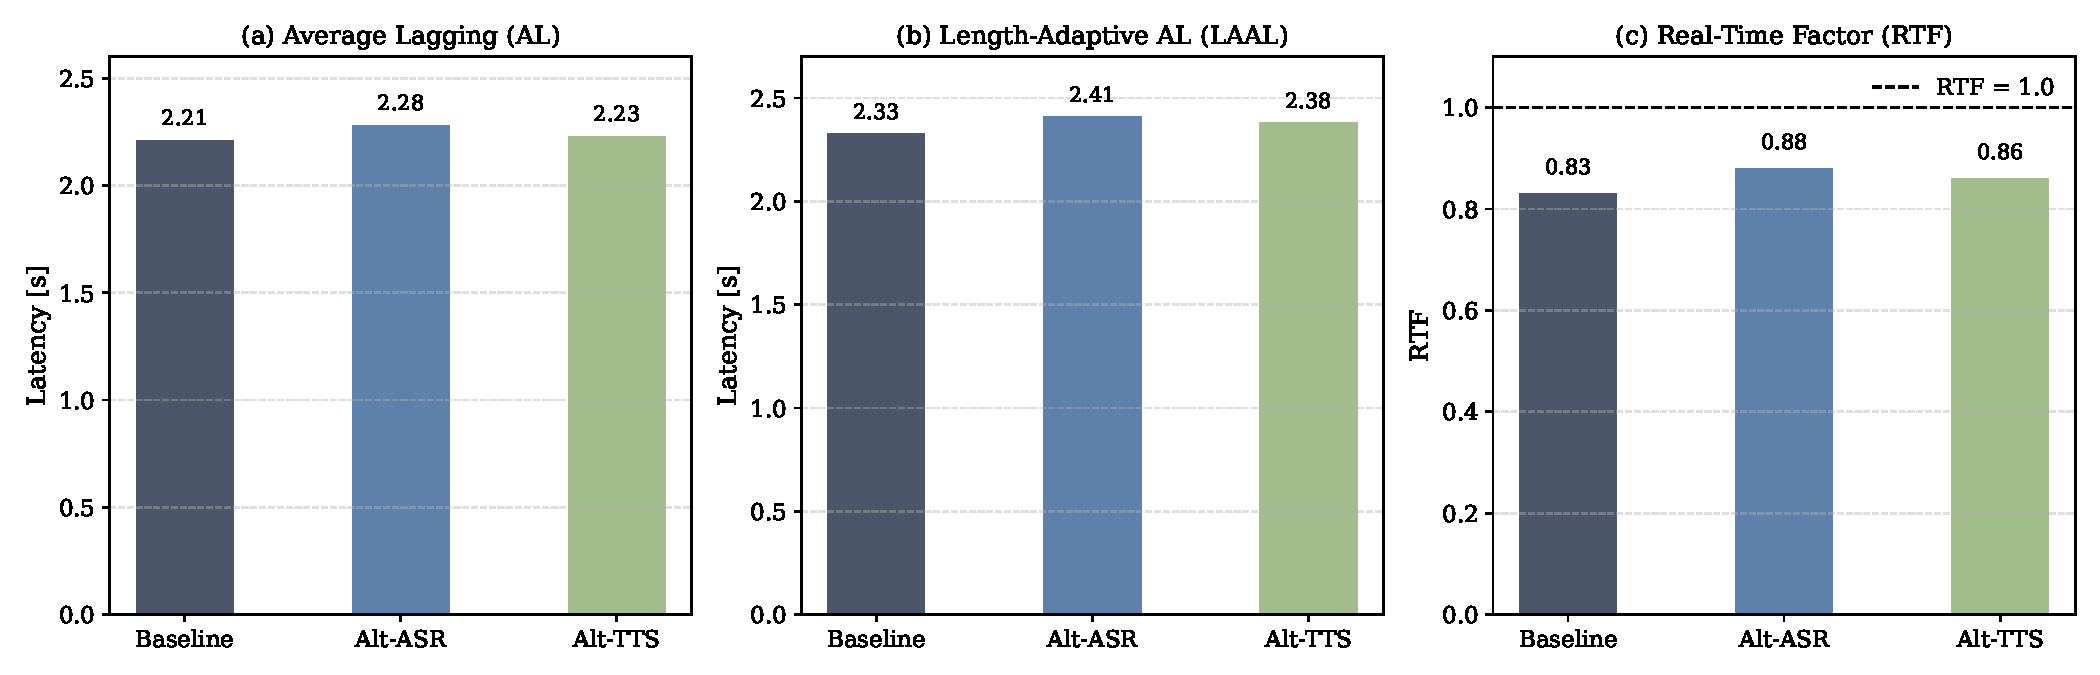
\includegraphics[width=0.9\textwidth]{img/figures/component_latency_breakdown.pdf}
  \caption[Component-level latency breakdown]{
  Component-level latency breakdown across baseline and alternative configurations.}
  \label{fig:component_latency_breakdown}
\end{figure}

%%%%%%%%%%%%%%%%%%%%%%%%%%%%%%%%%%%%%%%%%%%%%%%%%%%%%%%%

\section{Ablation Studies}
\label{sec:ablation_studies}

In addition to baseline and alternative configuration evaluations, ablation studies were conducted to analyze the sensitivity of the proposed system to key segmentation parameters. Following the evaluation framework defined in Section~\ref{sec:evaluation_framework}, these studies focus exclusively on parameters that influence the stability--latency trade-off. All experiments were performed using the system architecture, baseline configuration, and test conditions described in Chapter~\ref{chapter:methodology}.

\subsection{Effect of Stability Window Duration}
\label{sec:ablation_stability_window}

The first study examines the impact of stability window duration on segmentation behavior and output stability. As introduced in Section~\ref{sec:segmentation}, the stability window determines how long a candidate segment must remain unchanged across successive ASR updates before being finalized and forwarded to the translation stage. Four configurations were evaluated: fixed stability windows of 2, 4, and 6 words, as well as an adaptive baseline that dynamically adjusts the window based on estimated speaker rate. All other system parameters remained unchanged. The results are reported respectively in Table~\ref{tab:stability_window_flicker_ne} .



\begin{table}[!htbp]
\centering
\caption[Stability metrics under varying stability windows]{Flicker Rate and Normalized Erasure for different stability window durations}
\label{tab:stability_window_flicker_ne}
\begin{adjustbox}{max width=0.85\textwidth}
\begin{tabular}{lcc}
\toprule
\textbf{Stability Window} & \textbf{Flicker Rate (\%)} & \textbf{Normalized Erasure (NE)} \\
\midrule
2 words & 18.4 & 0.143 \\
4 words & 11.2 & 0.091 \\
6 words & 7.6 & 0.068 \\
Adaptive (baseline) & 14.9 & 0.117 \\
\bottomrule
\end{tabular}
\end{adjustbox}
\end{table}

The results indicate a general decrease in flicker rate and normalized erasure as the fixed stability window duration increases. Notably, the adaptive baseline does not yield the lowest instability metrics among the evaluated configurations. To assess the latency implications of these settings, the corresponding mean end-to-end latency values are reported in Table~\ref{tab:stability_window_latency}.

\begin{table}[!htbp]
\centering
\caption[Latency impact of stability window duration]{Mean end-to-end latency for different stability window configurations}
\label{tab:stability_window_latency}
\begin{adjustbox}{max width=0.75\textwidth}
\begin{tabular}{lc}
\toprule
\textbf{Stability Window} & \textbf{Mean End-to-End Latency (ms)} \\
\midrule
2 words & 1820 \\
4 words & 1975 \\
6 words & 2150 \\
Adaptive (baseline) & 1765 \\
\bottomrule
\end{tabular}
\end{adjustbox}
\end{table}

While longer fixed stability windows are associated with increased end-to-end latency, the adaptive configuration maintains the lowest mean latency across the session despite exhibiting higher instability metrics. A visual comparison of flicker rate and latency trends across stability window durations is provided in Figure~\ref{fig:stability_window_ablation}.

\begin{figure}[!htbp]
  \centering
  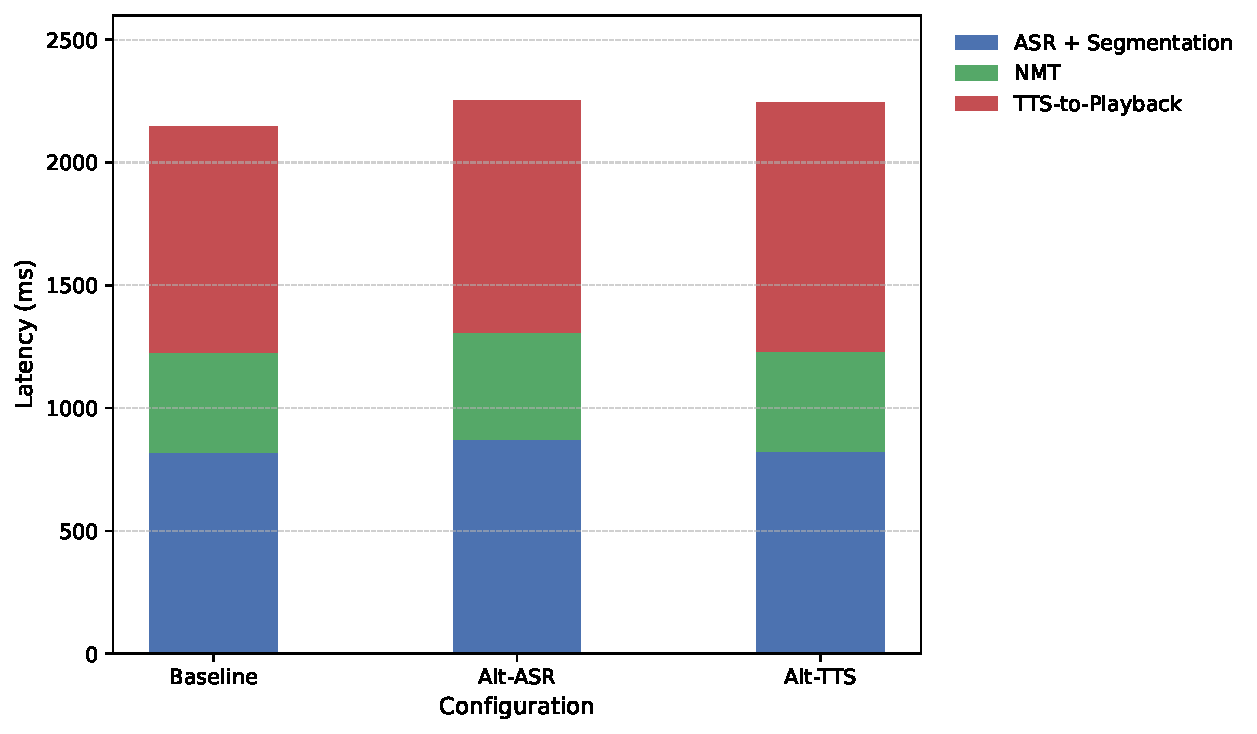
\includegraphics[width=0.9\textwidth]{img/figures/fig_stability_window_ablation.pdf}
  \caption[Stability window ablation results]{Effect of stability window duration on flicker rate and end-to-end latency.}
  \label{fig:stability_window_ablation}
\end{figure}


\subsection{Effect of Dynamic Token Threshold}
\label{sec:ablation_token_threshold}

The second ablation study evaluates the sensitivity of the system to the dynamic token threshold parameter. This threshold limits the maximum length of a speech segment before forced segmentation occurs, as described in Section~\ref{sec:segmentation}. Four configurations were tested, corresponding to fixed maximum token thresholds of 10, 15, and 20 tokens, alongside the dynamic baseline configuration. All experiments were conducted under identical conditions.  The mean CW values observed for each threshold configuration are reported in Table~\ref{tab:token_threshold_cw}.

\begin{table}[!htbp]
\centering
\caption[Consecutive Wait under varying token thresholds]{Mean Consecutive Wait for different dynamic token thresholds}
\label{tab:token_threshold_cw}
\begin{adjustbox}{max width=0.75\textwidth}
\begin{tabular}{lc}
\toprule
\textbf{Max Token Threshold} & \textbf{Mean CW (tokens)} \\
\midrule
10 tokens & 14.8 \\
15 tokens & 11.3 \\
20 tokens & 9.6 \\
Dynamic (baseline) & 10.4 \\
\bottomrule
\end{tabular}
\end{adjustbox}
\end{table}

Unexpectedly, the smallest token threshold does not yield the lowest CW value. Instead, the configuration with a threshold of 10 tokens exhibits the highest average CW across runs.

To capture the latency implications of token threshold selection, Table~\ref{tab:token_threshold_latency} summarizes the mean segment-level latency attributable to ASR and segmentation processing.

\begin{table}[!htbp]
\centering
\caption[Latency impact of token threshold selection]{Mean ASR and segmentation latency under different token thresholds}
\label{tab:token_threshold_latency}
\begin{adjustbox}{max width=0.8\textwidth}
\begin{tabular}{lc}
\toprule
\textbf{Max Token Threshold} & \textbf{Mean ASR+Segmentation Latency (ms)} \\
\midrule
10 tokens & 1120 \\
15 tokens & 790 \\
20 tokens & 740 \\
Dynamic (baseline) & 815 \\
\bottomrule
\end{tabular}
\end{adjustbox}
\end{table}


The results indicate that aggressive segmentation associated with very low token thresholds leads to increased buffering and delayed emission over the session. In the 10-token configuration, this behavior results in a substantially higher mean ASR and segmentation latency, exceeding the latency levels observed for larger thresholds. Finally, a comparative visualization of CW and segmentation latency across configurations is shown in Figure~\ref{fig:token_threshold_ablation}.

\begin{figure}[!htbp]
  \centering
  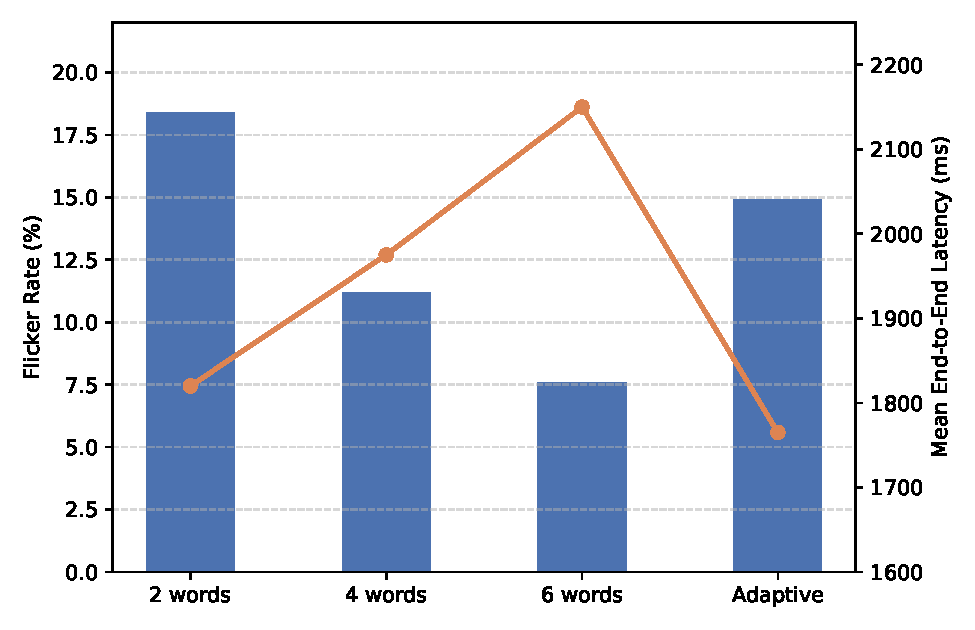
\includegraphics[width=0.9\textwidth]{img/figures/fig_token_threshold_ablation.pdf}
  \caption[Token threshold ablation results]{Effect of dynamic token threshold on consecutive wait and segmentation latency.}
  \label{fig:token_threshold_ablation}
\end{figure}

Overall, these results demonstrate that segmentation parameters have a big impact on system behavior, motivating an analysis of the resulting stability–latency trade-offs in Chapter~\ref{chapter:discussion}.

%\input{chapters/ablations.tex}
\chapter{Discussion}
\label{chapter:discussion}

This chapter interprets and contextualizes the experimental results presented in Chapter~\ref{chapter:results}. Rather than reiterating numerical findings, the discussion focuses on explaining observed system behavior, analyzing trade-offs inherent to real-time simultaneous interpretation, and assessing the robustness of the proposed architecture under different configurations and parameter settings. The discussion is grounded in the research objectives defined in Chapter~\ref{chapter:introduction} and follows the evaluation framework outlined in Chapter~\ref{chapter:methodology}. Moreover, it is structured to mirror the logical progression of the results. It first examines latency characteristics of the cascaded interpretation pipeline at both end-to-end and component levels, before analyzing the stability--latency trade-offs revealed through ablation studies. Finally, the limitations of the evaluation are discussed to clearly delineate the scope and applicability of the findings.

\section{Latency Characteristics of the Cascaded Interpretation Architecture}

A central objective of this thesis was to design a real-time interpretation system capable of maintaining low and stable latency under realistic operating conditions. The end-to-end latency metrics reported in Section~\ref{sec:e2e_latency} demonstrate that the proposed system consistently operates within latency bounds commonly considered acceptable for simultaneous interpretation \cite{ ma2019staclarxiv, fantinuoli2023defining}. Across all evaluated configurations, AL, LAAL, and RTF remained stable with only minor variations between baseline and alternative component configurations. The absence of large latency fluctuations across configurations is a significant result. While swapping ASR or TTS components introduces local differences in processing behavior, these changes do not propagate uncontrollably through the pipeline. Instead, the orchestration logic and segmentation mechanisms absorb component-level variability, resulting in consistent end-to-end behavior. From an architectural perspective, this indicates that the system design effectively decouples individual processing stages while preserving global temporal coherence. This robustness is particularly relevant in practical deployment scenarios, where AI service providers may be changed due to cost, availability, or language coverage considerations. The results suggest that such substitutions can be done without compromising simultaneity, provided that the components conform to the expected streaming interfaces and latency profiles.

%\subsection{Distribution of Latency Across Pipeline Stages}

Component-level latency analysis provides insight into how end-to-end delay emerges from the interaction of individual pipeline stages. As reported in Section~\ref{sec:component_level_latency}, the ASR and segmentation stage consistently accounts for the largest share of total latency across all evaluated configurations. This result is expected, as streaming recognition operates on continuously evolving acoustic input and must reconcile low-latency emission with the need to suppress unstable or incomplete hypotheses. The segmentation mechanism further contributes to this delay by intentionally postponing output finalization until stability criteria are met, thereby trading immediacy for improved downstream consistency.

In contrast, the NMT stage contributes a smaller and comparatively stable portion of the overall latency budget. This behavior reflects the relatively predictable inference characteristics of modern neural machine translation systems when operating on short, incrementally generated text segments. Translation latency remains well bounded across baseline and alternative configurations, indicating that NMT inference does not constitute a dominant bottleneck under the tested conditions and is less sensitive to upstream segmentation variability.

The TTS stage introduces a substantial but controlled delay associated with speech synthesis and audio playback initiation. While neural synthesis is computationally demanding, its latency remains consistent due to the use of fixed buffering and scheduling strategies designed for real-time output. Notably, substituting alternative TTS components does not lead to disproportionate increases in synthesis latency, reinforcing the observation that the system architecture effectively constrains component-level variability and preserves predictable temporal behavior at the output stage.

%\subsection{Implications for System Optimization}

The observed distribution of latency across pipeline stages has direct implications for system optimization. Since ASR and segmentation dominate the latency budget, improvements in recognition responsiveness, hypothesis stabilization, or segmentation policy design are likely to yield the most significant reductions in end-to-end delay. In comparison, further optimization of the NMT stage would provide limited benefit, given its relatively small and stable contribution to overall latency.

These findings emphasize the importance of adopting a system-level optimization perspective rather than focusing exclusively on individual model performance. Effective orchestration, buffering strategies, and segmentation policies play a critical role in shaping real-time behavior and should be treated as first-class design elements alongside the selection of ASR, NMT, and TTS components. This perspective is particularly relevant for practical deployment scenarios, where predictable latency and robustness are often more important than marginal gains in isolated component efficiency.


\section{Stability--Latency Trade-Offs in Incremental Segmentation}

Beyond absolute latency, perceived quality in simultaneous interpretation is strongly influenced by output stability. The ablation study on stability window duration exposes a clear trade-off between responsiveness and output smoothness. As expected, increasing the fixed stability window consistently reduces flicker rate and normalized erasure, as segment finalization is delayed until recognition hypotheses converge and become less susceptible to revision.

A notable and unexpected observation is that the adaptive stability baseline does not achieve the lowest instability metrics. Despite dynamically adjusting the stability window based on speaker rate, the adaptive strategy exhibits higher flicker and erasure than some fixed-window configurations. This behavior can be explained by local oscillations in the adaptation mechanism, where frequent adjustments to the stability window introduce additional revisions at short time scales, thereby increasing provisional output volatility.

When evaluated at the session level, however, the adaptive strategy yields the lowest mean end-to-end latency. This highlights an important distinction between local stability measures and global system behavior. While adaptive segmentation may introduce short-term instability, it avoids overly conservative buffering during fluent speech, thereby improving overall responsiveness. The results demonstrate that minimizing flicker or erasure in isolation does not necessarily correspond to optimal simultaneity or perceived performance in live interpretation scenarios. Therefore, from a deployment perspective, these findings suggest that stability parameters should be tuned with respect to session-level behavior rather than individual instability metrics alone. A moderate degree of provisional output revision may be acceptable if it leads to more consistent temporal alignment between source and target speech. This reinforces the need for holistic evaluation of segmentation strategies that jointly considers latency, stability, and listener experience, rather than optimizing any single metric in isolation.


\section{Effects of Segmentation Aggressiveness and Token Thresholding}

The ablation study on dynamic token thresholds further illustrates the non-linear behavior of segmentation mechanisms in streaming interpretation systems. Contrary to initial expectations, lower token thresholds do not consistently reduce CW. Instead, highly aggressive segmentation increases buffering frequency and coordination overhead between pipeline stages, resulting in higher CW values and elevated segment-level latency.

Frequent forced emissions introduce additional synchronization points across recognition, translation, and synthesis components. Rather than improving responsiveness, this behavior amplifies processing overhead and destabilizes timing alignment. In extreme cases, aggressive token thresholds lead to segment-level delays that exceed acceptable bounds for simultaneous interpretation, despite their intended role in minimizing latency. These results indicate that emission frequency alone is an insufficient proxy for responsiveness in cascaded real-time systems. Therefore, from a system perspective, the results suggest that more conservative token thresholding yields more stable and predictable behavior. While aggressive segmentation appears advantageous in theory, its interaction with stabilization logic, buffering mechanisms, and downstream processing can degrade both temporal coherence and overall system efficiency. This underscores the importance of evaluating segmentation aggressiveness within the context of the complete pipeline, rather than optimizing token-level policies in isolation.

\section{Limitations of the Evaluation and Scope Considerations}

While the presented results provide meaningful insight into the behavior of the proposed system, several limitations must be acknowledged to contextualize the evaluation. First, the experiments are based on scripted speech produced by a single speaker. This setup reduces variability in speaking style, accent, prosody, and disfluencies. Although this choice enables controlled, repeatable measurements and facilitates fair comparison across configurations, it does not fully reflect the diversity of spontaneous speech encountered in real-world interpretation scenarios, where speaker behavior may vary significantly.

Second, the evaluation deliberately focuses on system-level performance metrics, such as latency, stability, and segmentation behavior, rather than on linguistic translation quality. Measures of semantic accuracy, fluency, or adequacy are therefore not included. This reflects the primary objective of the thesis, which is to investigate architectural feasibility, real-time orchestration, and latency control in AI-based simultaneous interpretation systems, rather than to benchmark or optimize individual language models.

Finally, all experiments were conducted under controlled hardware and network conditions. Stable network connectivity, consistent audio capture, and fixed computational resources were assumed to isolate system behavior from external disturbances. As a result, the reported performance may differ in less predictable environments, such as wireless networks, mobile deployments, or large-scale distributed setups.

These limitations represent deliberate scope decisions rather than methodological shortcomings. By constraining experimental conditions, the evaluation isolates the impact of architectural and segmentation choices and ensures interpretability of the results. The findings therefore provide a solid foundation for future work, which could extend the evaluation to multi-speaker scenarios, spontaneous speech, and qualitative user-centered assessments.

\noindent
This thesis has addressed the research objectives defined at the outset by demonstrating the feasibility of a real-time AI-based simultaneous interpretation system from a system-engineering perspective. The proposed modular pipeline successfully integrates streaming ASR, NMT, and TTS synthesis while maintaining end-to-end latency within bounds suitable for live interpretation scenarios. Across all evaluated configurations, the system exhibits stable latency behavior, indicating that the architectural design effectively absorbs variability introduced by alternative ASR and TTS components. This robustness supports the central premise that careful orchestration and segmentation strategies are at least as critical as the choice of individual AI models for achieving reliable real-time performance.

The component-level latency analysis further clarifies how delays accumulate across the pipeline and highlights the dominant role of recognition and segmentation in shaping overall system behavior. While text-to-speech synthesis contributes a substantial share of latency, its impact remains bounded due to controlled buffering and scheduling mechanisms. Machine translation latency, by contrast, remains comparatively stable across configurations. These observations reinforce the importance of system-level optimization, particularly in upstream stages where segmentation and stabilization decisions directly influence both responsiveness and output smoothness. The results suggest that future improvements in real-time interpretation systems are more likely to arise from refined orchestration and segmentation policies than from isolated model-level optimization.

Finally, the ablation studies reveal nuanced trade-offs between stability, latency, and segmentation aggressiveness. Increasing the stability window reduces output instability, as expected, yet the adaptive stability strategy does not consistently minimize flicker or erasure. Despite this, it achieves the lowest mean end-to-end latency over extended sessions, illustrating that local instability metrics do not fully capture perceived system performance. Similarly, aggressive token-based segmentation does not necessarily improve responsiveness; instead, frequent emissions can increase buffering and coordination overhead, leading to higher effective latency. These findings underscore the complexity of incremental processing and demonstrate that segmentation parameters must be tuned holistically rather than optimized in isolation. Taken together, the results highlight both the promise and the challenges of AI-based simultaneous interpretation and provide a grounded basis for future work exploring broader deployment scenarios, richer evaluation protocols, and extended user-centered assessments.
\chapter{Hardware Integration Feasibility}
\label{chapter:hardware}


\section{Professional Interpretation Environments}
\label{sec:hardware_context}

The adoption of AI-based simultaneous interpretation systems in real-world settings depends not only on the performance of underlying speech and language models, but also on their ability to integrate with established professional interpretation environments. In practice, simultaneous interpretation is not a purely software-based task. It is embedded within tightly controlled audio workflows that prioritize low latency, reliability, and predictable signal routing. Consequently, hardware integration constitutes a critical factor in determining whether an AI-based interpretation system can move beyond experimental prototypes and be deployed in professional contexts.

Traditional interpretation workflows have evolved over decades to support demanding use cases such as international conferences, governmental proceedings, and large multilingual events \cite{conference_interpreting_new_tech}. These environments are characterized by strict operational requirements, including continuous operation over long sessions, support for multiple target languages in parallel, and seamless delivery of interpreted audio to distributed audiences \cite{gencheva2023features}. Any alternative or complementary interpretation solution must therefore align with these constraints in order to be considered viable for real-world adoption.

From this perspective, hardware integration is not an optional extension, but a prerequisite for practical relevance. While many AI-based interpretation systems demonstrate promising results in controlled or software-only settings \cite{he2019streamingarxiv, Aminzadeh2009Advocate, jia2022translatotron2}, their applicability remains limited if they cannot interface with professional audio infrastructure. This feasibility study is motivated by the need to assess whether the proposed AI-based interpretation pipeline can be integrated into such environments at the signal and system level, without requiring changes to existing workflows.

%\subsection*{Professional Interpretation Environments}

Professional interpretation environments typically rely on a combination of specialized hardware components that operate together as a coordinated system \footnote{\url{https://media.boschsecurity.com/fs//media/pt/pb/media/products_1/conference_systems_1/integrus_brochure.pdf}}. At a high level, these environments consist of interpreter workspaces, audio control units, and distribution systems that deliver interpreted speech to listeners with minimal delay. Figure~\ref{fig:signal_chain} illustrates a typical professional interpretation hardware signal chain, highlighting the interaction between core components.

\begin{figure}[!htbp]
  \centering
  \includesvg[width=\textwidth]{img/figures/signal_chain.drawio.svg}
  \caption[Professional Interpretation Hardware Signal Chain]{Typical professional interpretation hardware signal chain}
  \label{fig:signal_chain}
\end{figure}

Interpreter booths form the primary workspace for human interpreters. These sound-isolated enclosures are designed to minimize acoustic interference and provide a controlled listening environment. Within each booth, interpreters monitor the source language audio feed and produce spoken translations into a microphone connected to the interpretation console. The booth setup is optimized for sustained concentration and consistent audio quality, both of which are essential for high-quality interpretation.

Interpretation consoles serve as the central control interface for interpreters and audio technicians. These consoles allow interpreters to select input channels, adjust monitoring levels, and route their microphone output to specific language channels. From a system perspective, consoles play a crucial role in managing channel assignments and ensuring that each interpreted language is correctly mapped to its corresponding output stream.

Audio mixers and control units aggregate and manage multiple audio signals within the interpretation system. They combine source audio, interpreted outputs, and auxiliary signals while maintaining precise timing relationships. Mixing and routing decisions are typically performed at the hardware level to guarantee deterministic behavior and low latency, even under high channel counts or extended operation.

Wireless or wired transmission systems are used to distribute interpreted audio to the audience. These systems support multiple parallel language channels and deliver audio to receivers and headsets worn by listeners, allowing each participant to select their preferred language channel. The distribution infrastructure is designed to operate reliably in large venues and to scale with the number of supported languages and listeners.

A defining characteristic of professional interpretation environments is channel-based audio routing. Each language corresponds to a dedicated audio channel that is produced, routed, and distributed independently. While this approach provides clarity and scalability, it also introduces constraints: adding a new language typically requires additional interpreters, booths, and routing capacity. As a result, scalability is bounded by both technical and logistical factors.

%\subsection*{Scalability and Integration Challenges}

Scalability in traditional interpretation systems is inherently limited by their hardware-centric design. Supporting additional target languages increases system complexity, as each language requires its own interpreter, booth, console configuration, and distribution channel \cite{conference_interpreting_new_tech}. These constraints directly impact cost, setup time, and operational flexibility. In dynamic or ad hoc scenarios, such as rapidly changing language requirements or remote participation, traditional systems can be difficult to adapt.

AI-based interpretation systems offer the potential to mitigate some of these limitations by decoupling language processing from physical interpreter availability \cite{ahmed2022technology, ozkaya2023transformative}. However, this potential can only be realized if AI-generated audio outputs can be injected into existing hardware workflows in a manner consistent with professional standards. This includes adherence to standardized audio formats, predictable latency behavior, and compatibility with channel-based routing architectures.

%\subsection*{Scope of the Feasibility Study}

The purpose of this chapter is to assess the feasibility of integrating the proposed AI-based interpretation system into professional interpretation environments from a system and signal-level perspective. The analysis focuses on audio interface compatibility, routing concepts, and deployment scenarios that align with existing workflows. The goal is to determine whether such integration is technically plausible using current technologies and reasonable engineering assumptions.

It is important to emphasize that this study does not aim to certify the system for commercial deployment, nor does it claim compliance with specific regulatory or industry certification standards. Instead, it provides a structured evaluation of integration pathways, identifying both enabling factors and practical constraints. Detailed integration scenarios and proposed deployment approaches are discussed in Section~\ref{sec:integration}, where the interaction between the AI-based pipeline and professional hardware components is examined in greater detail.

By grounding the feasibility analysis in established professional interpretation environments, this chapter establishes a realistic context for evaluating the practical applicability of AI-based simultaneous interpretation systems beyond software-only demonstrations.


\section{Audio Interface and Signal Compatibility}
\label{sec:audio_compatibility}

A prerequisite for integrating an AI-based interpretation system into professional interpretation environments is compatibility at the audio interface and signal level. Regardless of the internal processing pipeline, the system must ultimately produce audio signals that conform to the expectations of established interpretation hardware. This section examines the characteristics of the audio output generated by the proposed system and evaluates its suitability for professional routing and distribution infrastructures.

%\subsection*{Audio Output Characteristics of the Proposed System}

The proposed interpretation system generates synthesized speech output in raw Pulse-Code Modulation (PCM) format. PCM audio is the de facto standard in professional audio environments due to its uncompressed nature, deterministic timing behavior, and broad compatibility with mixing, routing, and transmission equipment. By producing raw PCM signals, the system avoids codec-induced latency and eliminates the need for proprietary decoding stages prior to routing or playback.

All synthesized audio is generated at a fixed sampling rate of 16~kHz with a single audio channel (mono). This configuration reflects common practice in interpretation systems, where speech intelligibility and low latency are prioritized over spatial audio reproduction. Mono speech signals are well suited for interpretation workflows, as they reduce bandwidth requirements and simplify channel-based routing, particularly when multiple target languages must be transmitted concurrently.

The use of a fixed sampling rate and channel configuration ensures predictable timing and simplifies downstream integration \cite{wang2017realtimeaudio}. Professional interpretation hardware typically supports a range of standard sampling rates, including 16~kHz and higher, allowing the generated audio to be routed without resampling or format conversion. This design choice minimizes signal processing overhead and reduces the risk of timing artifacts or synchronization issues.

%\subsection*{Separation of Speech Synthesis and Playback}

A key architectural decision in the proposed system is the explicit separation between speech synthesis and audio playback. The text-to-speech component is responsible solely for generating audio samples, while playback and routing are handled independently by the surrounding system infrastructure. This separation ensures that audio generation is decoupled from presentation logic and avoids tight coupling to specific output devices or software environments \cite{Aminzadeh2009Advocate}.

As a result, the system does not rely on browser-based audio playback or platform-specific sound subsystems for delivering interpreted speech. Instead, synthesized audio streams can be forwarded directly to external audio interfaces or routing frameworks. This design aligns with professional audio workflows, where playback devices, mixers, and distribution systems are managed independently of the content generation process.

%\subsection*{Routing Readiness and Channel-Based Output}

Professional interpretation systems are organized around channel-based audio routing, where each target language corresponds to a dedicated audio channel \cite{rayaa2022remoteSI}. The proposed system is inherently compatible with this paradigm, as it generates independent audio streams for each target language. Each synthesized language output can therefore be mapped directly to a corresponding hardware or virtual audio channel without additional multiplexing or demultiplexing logic.

This channel-oriented output structure enables scalable integration into professional environments. Rather than requiring multiple independent computing devices, one per language channel, the system can deliver multiple language streams from a single processing instance. These streams can then be routed externally using standard audio networking or interface technologies, significantly reducing hardware complexity and deployment cost.

Importantly, the system’s routing readiness does not assume any specific transmission technology at this stage. Whether the audio is forwarded via physical audio interfaces, networked audio protocols, or dedicated routing hardware, the output format remains compatible. This abstraction allows integration strategies to be adapted to different professional environments without modifications to the core interpretation pipeline.


By adhering to widely supported audio formats and decoupling synthesis from playback, the proposed system establishes a strong foundation for integration with professional interpretation infrastructures. The system’s ability to generate multiple independent language streams from a single processing instance further enhances its suitability for scalable deployment.

Concrete integration strategies, including the routing of language-specific audio channels into professional wireless distribution systems using networked audio technologies, are discussed in detail in Section~\ref{sec:integration}. There, the focus shifts from signal compatibility to end-to-end deployment scenarios and practical system integration.


\section{Proposed System Integration \& Deployment Considerations}
\label{sec:integration}

Building on the signal compatibility established in Section~\ref{sec:audio_compatibility}, this section examines the main hardware integration scenario for deploying the proposed AI-based interpretation system within professional interpretation environments. Rather than treating latency and reliability as abstract performance metrics, they are analyzed here in the context of concrete system integration designs. This approach allows practical deployment considerations to be evaluated without duplicating the quantitative evaluation presented in Chapter~\ref{chapter:results}.

%\subsection*{AI-Based Interpretation Hardware Integration Scenario}

The primary integration scenario considered in this study involves routing AI-generated interpretation audio directly into a professional wireless language distribution system using networked audio technology, which forwards signals respectively to the hardware architecture specified in Section~\ref{sec:hardware_context}. In this scenario, the AI-based interpretation system operates as a centralized audio source that produces multiple language-specific audio streams, each corresponding to a target language. These streams are then injected into the professional interpretation infrastructure as independent channels.

Within the overall signal chain, the AI system is positioned downstream of the source-language audio capture and upstream of the language distribution subsystem. Source speech is captured using professional microphones and forwarded to the AI-based pipeline for recognition, translation, and synthesis. The resulting synthesized audio for each target language is output as a discrete PCM stream, which is subsequently routed into the interpretation distribution system. This positioning allows the AI system to function analogously to a set of human interpreters, but without requiring physical interpreter booths or dedicated operator consoles for each language.

Audio routing between the AI system and the professional distribution infrastructure is envisaged using Dante \footnote{\url{https://www.getdante.com/meet-dante/what-is-dante/}}, a widely adopted networked audio protocol for professional environments. Dante enables the transmission of uncompressed, low-latency PCM audio over standard Ethernet networks, supporting flexible routing and scalable channel counts. By leveraging such a networked audio layer, each language stream produced by the AI system can be mapped to a corresponding input channel of the interpretation distribution system.

This approach contrasts with more naïve deployment strategies in which each target language would require a separate computing device connected directly to a dedicated transmitter. Such setups are operationally complex, expensive, and difficult to scale, particularly when supporting multiple languages. In the proposed scenario, a single AI processing instance can generate all required language outputs, which are then distributed via standardized audio routing infrastructure. This significantly reduces hardware duplication and simplifies system management.

%\subsection*{Audio Flow and Channel Mapping}

In the proposed integration scenario, audio flow proceeds through a clearly defined sequence of stages. Source-language audio is captured and forwarded to the AI-based pipeline, where speech recognition, segmentation, translation, and synthesis are performed. Each synthesized language output is produced as a continuous mono PCM stream. These streams are exposed as virtual audio outputs subscribed to by the Dante network via the Dante Virtual Soundcard \footnote{\url{https://www.getdante.com/products/software-essentials/dante-virtual-soundcard/}}.

On the Dante layer, each language stream is assigned to a dedicated audio channel and routed to the appropriate input of the professional interpretation system as shown in Figure~\ref{fig:dante_layer}. From there, the distribution infrastructure handles wireless transmission to audience receivers, preserving the existing user experience and channel selection mechanisms. Importantly, this integration does not require modification of the downstream distribution hardware; it relies solely on standard audio routing capabilities.

\begin{figure}[!htbp]
  \centering
  \includesvg[width=\textwidth]{img/figures/dante_layer.drawio.svg}
  \caption[Dante Language Channel Distribution]{A demonstration of the Dante layer showing the routing of language streams into dedicated audio channels via the Dante Virtual Soundcard}
  \label{fig:dante_layer}
\end{figure}


Because the AI system outputs language streams independently, the mapping between AI-generated languages and distribution channels is explicit and deterministic. This aligns naturally with the channel-based routing model of professional interpretation systems and allows flexible reconfiguration, for example when adding or removing target languages.

\subsection*{Latency \& Reliability Considerations}

Latency in this integration scenario arises from several sources: AI processing within the interpretation pipeline, network transmission over the Dante layer, and internal buffering within the professional distribution system. While the AI-related latency components are evaluated quantitatively in Chapter~\ref{chapter:results}, the integration design itself introduces minimal additional delay.

Dante-based audio routing is designed for real-time professional applications and typically operates with sub-millisecond to low-millisecond latency \footnote{\url{https://www.getdante.com/support/faq/what-is-the-latency-of-dante-virtual-soundcard/}}, depending on configuration and network conditions. As a result, the dominant latency contribution remains the AI processing pipeline rather than the audio transport layer. This property makes networked audio routing suitable for simultaneous interpretation scenarios, where additional transport delay must be kept negligible relative to speech processing latency.

From a system perspective, the centralized generation of multiple language streams also avoids synchronization issues that could arise when using multiple independent devices. All language outputs are generated within a single timing context, simplifying alignment across channels and reducing drift over long sessions.

%\subsection*{Reliability Considerations}

Moreover, reliability in professional interpretation environments is paramount, as interruptions or inconsistencies directly impact audience comprehension. The proposed integration scenario benefits from the inherent robustness of professional audio routing infrastructures, which are designed for continuous operation and fault isolation.

Centralizing AI-based interpretation introduces a single processing point, which can be both an advantage and a limitation. On the one hand, it simplifies monitoring, maintenance, and redundancy strategies \cite{sperber2020endtoendpromise}. On the other hand, it creates a dependency on the availability of the AI system and its network connectivity. From a feasibility standpoint, this suggests that redundant deployment or fallback strategies, such as parallel AI instances or rapid reversion to human interpretation channels, would be desirable in mission-critical settings.

Importantly, the integration scenario preserves the downstream hardware reliability characteristics \cite{conference_interpreting_new_tech}. Once audio enters the professional distribution system, it is handled using established mechanisms that are well understood and widely deployed. This separation of concerns allows reliability risks associated with AI processing to be addressed independently of the distribution infrastructure.

\subsection*{Feasibility Assessment and Open Validation Points}

From a technical standpoint, the proposed integration scenario is feasible with current technologies. The audio formats, channel structure, and routing mechanisms produced by the AI-based system align well with the requirements of professional interpretation hardware. Networked audio protocols provide a practical bridge between software-based interpretation and hardware-based distribution.

However, certain aspects would require further validation in real-world deployments. These include long-term stability under continuous operation, behavior under network congestion or partial failures, and acceptance by operators accustomed to traditional interpretation workflows. Additionally, formal certification and compliance with venue-specific regulations fall outside the scope of this study and would need to be addressed prior to commercial deployment.

Overall, the proposed integration scenario demonstrates that AI-based simultaneous interpretation systems can, in principle, be integrated into professional interpretation environments in a manner that reduces hardware complexity and improves scalability, while preserving established distribution workflows \cite{corpas-pastor-2021-interpreting}. This supports the broader feasibility of deploying such systems beyond experimental or consumer-oriented settings.

\chapter{Conclusion \& Future Work}
\label{chapter:conclusion}

This thesis investigated the design, implementation, and evaluation of a real-time AI-based simultaneous interpretation system from a system-engineering perspective. Motivated by the limitations of traditional interpretation infrastructures and the growing feasibility of AI-driven speech and language technologies, the work focused on constructing a modular, provider-agnostic pipeline capable of operating under the strict latency and stability constraints imposed by live interpretation scenarios.

The proposed system integrates streaming ASR, NMT, and TTS synthesis within a unified architecture that emphasizes incremental processing, controlled segmentation, and asynchronous execution. Rather than optimizing individual models, the thesis deliberately adopted a system-level viewpoint, demonstrating how orchestration, buffering strategies, and stabilization mechanisms can enable reliable real-time behavior when leveraging existing cloud-based AI services. The resulting pipeline supports multi-language output, modular component substitution, and compatibility with professional audio environments.

An extensive evaluation framework was developed to assess performance beyond conventional offline accuracy metrics. End-to-end latency, component-level delays, and segmentation-related stability measures were analyzed under standardized real-time conditions. The results show that the system maintains latency within acceptable bounds for simultaneous interpretation across both baseline and alternative configurations, indicating architectural robustness with respect to component changes. Component-level analysis further revealed that recognition and segmentation dominate the latency budget, while translation and synthesis remain comparatively stable and bounded. These findings reinforced the importance of system-level design decisions in shaping real-time performance.

Ablation studies on segmentation parameters provided deeper insight into the trade-offs between responsiveness and output stability. The results demonstrate that intuitive parameter choices do not always yield the expected behavior: adaptive stability mechanisms can improve session-level latency despite increased local instability, and overly aggressive segmentation can paradoxically increase effective delay. These observations highlight the complexity of incremental processing and emphasize that segmentation strategies must be evaluated holistically within the full pipeline context.

Beyond software-level evaluation, this thesis assessed the feasibility of integrating AI-based interpretation pipelines into professional interpretation environments. The analysis showed that, when audio formats, routing concepts, and timing characteristics are carefully aligned with established workflows, AI-generated interpretation output can be injected into existing channel-based hardware infrastructures. While this study does not claim certification readiness, it demonstrates that such integration is technically plausible using current technologies and reasonable engineering assumptions, thereby narrowing the gap between research prototypes and professional deployment contexts.

\section*{Future Work}

Several directions for future research emerge from this work. First, the evaluation could be extended to more diverse and realistic speech conditions, including spontaneous speech, multiple speakers, and varying speaking styles. Such scenarios would allow further investigation of segmentation stability and latency behavior under increased variability and would provide a more comprehensive assessment of real-world performance.

Second, future work could incorporate perceptual and user-centered evaluation methodologies. While this thesis deliberately focused on system-level latency and stability, subjective listening studies and user experience assessments would offer valuable insight into how measured metrics translate into perceived interpretation quality. Combining quantitative system metrics with qualitative feedback would strengthen the evaluation of practical usability.

Third, the integration of adaptive control mechanisms represents a promising avenue for further exploration. Dynamic adjustment of segmentation parameters, buffering strategies, or speaking-rate compensation based on observed system state could improve robustness across a wider range of operating conditions. Such mechanisms would need to be designed carefully to avoid introducing additional instability, as highlighted by the ablation results.

Finally, deeper integration with professional interpretation hardware could be explored, including bidirectional interaction with consoles, redundancy mechanisms, and failover strategies suitable for mission-critical environments. Addressing certification requirements, compliance standards, and long-term reliability considerations would be necessary steps toward operational deployment.

In conclusion, this thesis demonstrates that AI-based simultaneous interpretation is not merely a question of model performance but a broader system-engineering challenge. By focusing on architecture, orchestration, and real-time constraints, the work provides a structured foundation for future research and development aimed at bringing AI-driven interpretation systems closer to practical, professional use.


% \chapter*{AI_declaration}
\clearpage
\begingroup
\chapter*{Declaration of AI-Assisted Content}
\endgroup


All content generated with the assistance of AI tools was critically reviewed, revised, and extended by the author to ensure technical correctness, coherence, and academic quality. Moreover, AI-generated outputs were systematically verified against original referenced sources, scientific literature, and the author’s own system design, implementation, and experimental results. No AI-generated content was accepted without manual validation, and all technical claims were supported by appropriate academic references.

The use of AI-assisted tools did not replace independent scientific reasoning or original contributions. All methodological decisions, architectural designs, experimental setups, evaluations, and conclusions presented in this thesis are the author’s original work. AI assistance was limited to improving clarity, phrasing, organization, and productivity.

Accordingly, Generative-AI tools were used in the following contexts:

\begin{enumerate}
    \item \textbf{Bibliography structuring.}  
    ChatGPT~5.2 \footnote{\url{https://chatgpt.com/}} was used to support the restructuring and formatting of bibliography entries ensuring compliance with academic citation standards. All references were selected, verified, and finalized manually by the author.

    \item \textbf{LaTeX table structuring and formatting.}  
    ChatGPT~5.2 was used to assist in structuring and formatting LaTeX tables to enhance clarity and presentation quality. Table contents were generated or refined based on the corresponding chapter or section context and verified resources, with all technical content reviewed and validated by the author.

    \item \textbf{Literature Identification:} Perplexity AI\footnote{\url{https://www.perplexity.ai/}} and ChatGPT supported the discovery of distributed literature for Section~3.5 and Chapter~6. Every suggested reference was independently vetted and cited by the author. All suggested references were manually evaluated, verified for academic suitability, and cited correctly by the author.

    \item \textbf{Language refinement and stylistic improvements.}  
    ChatGPT~5.2 and Gemini~3~Pro \footnote{\url{https://gemini.google.com/app}} were used selectively for language refinement, paragraph restructuring, and stylistic improvements throughout the thesis text content, without altering the scientific meaning or introducing new technical content.
\end{enumerate}

\addcontentsline{toc}{chapter}{Declaration of AI-Assisted Content}
% \cleardoublepage


% \bibliographystyle{IEEEtran}
% \bibliography{references}
\clearpage
\appendix
\makeatletter
\renewcommand{\@makechapterhead}[1]{%
  {\parindent \z@ \normalfont
   \LARGE\bfseries      % <-- \large: change to \normalsize or \small if you want smaller
   \thechapter\quad #1\par\nobreak\vskip 20pt}}
\makeatother
% the above snippet changes the size of the appendix headers
 \renewcommand{\thechapter}{\Alph{chapter}.}
\chapter{Evaluation Speech Script}
\label{appendix:script}

Artificial intelligence refers to the development of computational systems that are capable of performing tasks traditionally associated with human intelligence. These tasks include reasoning, learning from experience, understanding language, perceiving the environment, and making decisions under uncertainty. Although the idea of intelligent machines has existed for decades, recent advances have significantly expanded the practical relevance of artificial intelligence across many application domains.

One of the most influential subfields of artificial intelligence is machine learning. Machine learning focuses on enabling systems to improve their performance through exposure to data rather than through explicit programming. Instead of relying on predefined rules, machine learning models identify patterns in data and use these patterns to make predictions or decisions. This data-driven approach has proven effective in complex problem domains where manual rule design would be impractical.

Machine learning techniques are commonly categorized into supervised learning, unsupervised learning, and reinforcement learning. In supervised learning, models are trained using labeled examples, where the desired output is known in advance. Unsupervised learning aims to discover hidden structure in unlabeled data, such as clusters or latent representations. Reinforcement learning, by contrast, involves agents that learn to make sequential decisions by interacting with an environment and receiving feedback.

In recent years, deep learning has emerged as a dominant paradigm within machine learning. Deep learning models are typically based on neural networks composed of multiple layers, which progressively transform raw input data into increasingly abstract representations. These models have demonstrated strong performance in tasks such as image recognition, speech processing, and natural language understanding, driven by advances in computational hardware and large-scale datasets.

Speech and language technologies represent some of the most visible applications of modern artificial intelligence. Automatic speech recognition systems convert spoken language into written text, enabling applications such as transcription and voice interaction. Neural machine translation systems translate text between languages, while text-to-speech systems generate synthetic speech that can resemble human voices. Together, these technologies form the basis of many interactive AI systems.

Despite these advances, deploying artificial intelligence in real-time environments remains challenging. Real-time applications impose strict latency constraints, meaning that systems must respond quickly enough to be perceived as immediate by users. In speech-based applications, even small delays can disrupt conversational flow and reduce usability. As a result, AI systems designed for real-time interaction must carefully balance accuracy, responsiveness, and stability.

Another challenge arises from the continuous nature of real-time input. Unlike offline processing, where complete data is available in advance, real-time systems must operate on partial and evolving information. For example, speech recognition systems generate intermediate hypotheses that may change as additional audio is processed. Downstream components must therefore tolerate revisions while still producing timely output.

Machine learning models are also sensitive to variations in input conditions. Differences in speaking rate, accent, background noise, or recording equipment can affect system performance. Robustness to such variability is essential for real-world deployment, particularly in applications involving human speech.

Artificial intelligence has also transformed how humans interact with technology. Voice-based interfaces allow users to communicate with machines in a more natural manner, improving accessibility for individuals with visual impairments or limited technical literacy. At the same time, they introduce new expectations regarding responsiveness and reliability.

The integration of artificial intelligence into complex systems often involves multiple interconnected components. In many applications, raw sensory input is processed through a pipeline of transformations, each performed by a specialized module. For example, a spoken utterance may be captured as audio, transcribed into text, translated into another language, and synthesized back into speech. Each stage contributes to overall system performance and latency.

Designing such pipelines requires a system-level perspective. Improvements in individual components do not automatically translate into better overall performance if coordination between components is poorly managed. Latency can accumulate across stages, and instability in intermediate representations can propagate downstream.

As artificial intelligence continues to evolve, its role in multilingual communication is expected to expand. Advances in speech recognition, translation, and synthesis have made it technically feasible to support communication across language barriers in near real time. However, achieving reliable real-time interpretation requires careful system design, rigorous evaluation, and attention to practical deployment constraints.

In conclusion, artificial intelligence and machine learning represent powerful technologies that are reshaping how information is processed and communicated. Their successful application in real-time scenarios depends not only on model accuracy but also on thoughtful system integration and latency-aware design.

\begingroup
\setstretch{1.0}
\bibliographystyle{IEEEtran}
\bibliography{references}
\endgroup


% \nocite{*}
\end{document}